\documentclass{book}

% Configuration
% ------------------
% Packages
% ------------------
\usepackage[english]{babel}
\usepackage[T1]{fontenc}
\usepackage[scaled]{helvet}
\usepackage[utf8]{inputenc}
\usepackage[letterpaper]{geometry}
\usepackage[dvipsnames]{xcolor}

\usepackage{algorithmicx}
\usepackage{amsfonts,amsmath,amsthm,amssymb}
\usepackage{booktabs}
\usepackage{dsfont}
\usepackage{float}
\usepackage{graphicx}
\usepackage{latexsym}
\usepackage{mathtools}
\usepackage{sectsty}
\usepackage{setspace}
\usepackage{subcaption}
\usepackage{tabularx}
\usepackage{tikz}
\usepackage{tikz-3dplot}
% \usepackage{txfonts}
\usepackage{url}
\usepackage{wrapfig}
\usepackage{xparse}

% ------------------
% Shortcuts
% ------------------
\newcommand{\N}{\mathbb{N}}
\newcommand{\R}{\mathbb{R}}
\newcommand{\C}{\mathbb{C}}
\newcommand{\Z}{\mathbb{Z}}

\newcommand{\complexspace}[1]{\complexset^{#1}}
\newcommand{\realspace}[1]{\realset^{#1}}

\newcommand{\inverse}[1]{{#1}^{-1}}
\newcommand{\transpose}[1]{{#1}^{\top}}

\newcommand{\vdim}[1]{\mathrm{dim}\left( #1 \right)}
\newcommand{\vrank}[1]{\mathrm{rk}\left( #1 \right)}
\newcommand{\vspan}[1]{\mathrm{span}\left[ #1 \right]}

\newcommand{\id}{\mathrm{id}}
\newcommand{\GL}{\mathrm{GL}}
\newcommand{\sgn}{\mathrm{sgn}}

\newcommand{\im}[1]{\mathrm{Im}\left( #1 \right)}

\def\lcirclearrowleft{\ensuremath{%
  \rotatebox[origin=c]{180}{$\circlearrowleft$}}}
\def\lcirclearrowright{\ensuremath{%
  \rotatebox[origin=c]{180}{$\circlearrowright$}}}

\newcommand{\actson}{~\lcirclearrowright~}

% ------------------
% Command Redefinitions
% ------------------
\renewcommand{\qed}{\hfill$\blacksquare$}

\makeatletter
\renewcommand*\env@matrix[1][*\c@MaxMatrixCols c]{%
    \hskip -\arraycolsep
    \let\@ifnextchar\new@ifnextchar
    \array{#1}}
\makeatother

\renewcommand{\phi}{\varphi}
\renewcommand{\ker}[1]{\mathrm{ker}\left( #1 \right)}

% ------------------
% Colors
% ------------------
\definecolor{primary}{HTML}{207BA5}
\definecolor{greybg}{RGB}{249, 249, 249}

\definecolor{thmbg}{HTML}{F2F2F9}
\definecolor{lemmabg}{HTML}{FFFAF8}
\definecolor{lemmafr}{HTML}{983b0f}
\definecolor{propbg}{HTML}{f2fbfc}
\definecolor{propfr}{HTML}{191971}
\definecolor{myp}{RGB}{197, 92, 212}
\definecolor{grey17}{RGB}{17, 17, 17}
\definecolor{MyGrey}{HTML}{5B5B5B}

\definecolor{lightBlue}{rgb}{0.0, 0.64, 1.0}
\definecolor{lightRed}{rgb}{1.0, 0.50, 0.50}
\definecolor{darkGreen}{rgb}{0.31, 0.54, 0.30}
\definecolor{violet}{RGB}{186, 153, 242}

%----------------
%	Text Styles
%----------------
\DeclareTextFontCommand{\term}{\color{orange}\bfseries}
\DeclareTextFontCommand{\bred}{\color{red}\bfseries}
\DeclareTextFontCommand{\itblue}{\color{lightBlue}\itshape}

\DeclareTextFontCommand{\vector}{\bfseries\itshape}

% ------------------
%   URL Color
% ------------------
\usepackage[colorlinks=true]{hyperref}
\hypersetup{
    colorlinks=true,
    linkcolor=black,
    filecolor=magenta,
    urlcolor=blue,
}

% ------------------
% Tikz Externalize
% ------------------
\usetikzlibrary{external}
\tikzexternalize[prefix=tikz/]
\tikzset{external/only named=true}

% ------------------
% Boxes
% ------------------
\usepackage[most]{tcolorbox}

\newcommand\fancybox[3]{%
    \tcbset{
        mybox/.style={
                enhanced,
                boxsep=0mm,
                opacityfill=0,
                overlay={
                        \coordinate (X) at ([xshift=-1mm, yshift=-1.5mm]frame.north west);
                        \node[align=right, text=#1, text width=2.5cm, anchor=north east] at (X) {\bf#2};
                        \draw[line width=0.5mm, color=#1] (frame.north west) -- (frame.south west);
                    }
            }
    }
    \begin{tcolorbox}[mybox]
        #3
    \end{tcolorbox}
}

\tcbuselibrary{theorems,skins,hooks}
\NewDocumentCommand\thmbox{m O{\Large #1} O{greybg} O{primary} O{number within=section}}
{
    \newtcbtheorem[#5]{#1}{\large #2}
    {%
        enhanced,
        breakable,
        colback = #3,
        frame hidden,
        boxrule = 0sp,
        borderline west = {2pt}{0pt}{#4},
        sharp corners,
        detach title,
        before upper = \tcbtitle\par\smallskip,
        coltitle = #4,
        fonttitle = \bfseries,
        description font = \mdseries,
        separator sign none,
        segmentation style={solid, #4}
    }
    {th}
}

\thmbox{Corollary}[Corollary][myp!10][myp!85!black]
\thmbox{Lemma}[Lemma][lemmabg][lemmafr]
\thmbox{Propo}[Proposition][propbg][propfr]
\thmbox{Defi}[Definition][primary!12][primary]
\thmbox{Notation}[Notation][white][grey17][no counter]
\thmbox{Theorem}[Theorem][primary!12][primary]
\thmbox{Remark}[Remark][grey17!10][grey17][no counter]

% ------------------
% Environments
% ------------------
\newenvironment{corollary}[1][]   {\begin{Corollary}{#1}{}}                               {\end{Corollary}}
\newenvironment{definition}[1][]  {\begin{Defi}{#1}{}}                                    {\end{Defi}}
\newenvironment{lemma}[1][]       {\begin{Lemma}{#1}{}}                                   {\end{Lemma}}
\newenvironment{proposition}[1][] {\begin{Propo}{#1}{}}                                   {\end{Propo}}
\newenvironment{remark}[1][]      {\begin{Remark}{#1}{}}                                  {\end{Remark}}
\newenvironment{theorem}[1][]     {\begin{Theorem}{#1}{}}                                 {\end{Theorem}}

\newenvironment{rtheorem}[2][]    {\begin{Theorem}{#1}{#2}}                               {\end{Theorem}}

\theoremstyle{definition}
\newtheorem*{exam}{\color{primary}Example}
% \newcommand{\example}[1]{\begin{exam}#1\end{exam}}
% \newenvironment{example}          {\begin{exam}} {\begin{flushright}${\color{primary}\diamondsuit}$\end{flushright} \end{exam}}
\newenvironment{example}          {\begin{exam}} {\hfill${\color{primary}\diamondsuit}$\end{exam}}

\theoremstyle{definition}
\newtheorem*{clm}{\color{MyGrey}Claim}
\newenvironment{claim}            {\begin{clm}} {\end{clm}}

% ------------------
% Lists
% ------------------
\usepackage{enumitem}

\newcommand{\cnumero}[2]{
    \tikz[baseline=(myanchor.base)]
    \node[minimum size=0.2cm,circle,
        inner sep=1pt,draw, #2,thick,fill=#2](myanchor)
    {\color{white}\bfseries\fontsize{8}{8}#1};}

\newcommand*{\itembolasazules}[1]{\protect\cnumero{#1}{primary}}

\newenvironment{listo} {\begin{enumerate}[label=\itembolasazules{\arabic*}]} {\end{enumerate}}
\newenvironment{listu} {\begin{itemize}  [label=$\color{primary} \bullet$]}  {\end{itemize}}

% ------------------
% Table of Contents
% ------------------
\usepackage{blindtext}
\usepackage{framed}
\usepackage{titletoc}
\usepackage{etoolbox}

\patchcmd{\tableofcontents}{\contentsname}{\contentsname}{}{}

\renewenvironment{leftbar}
{\def\FrameCommand{\hspace{6em}%
        {\color{primary}\vrule width 2pt depth 6pt}\hspace{1em}}%
    \MakeFramed{\parshape 1 0cm \dimexpr\textwidth-6em\relax\FrameRestore}\vskip2pt%
}
{\endMakeFramed}

\titlecontents{chapter}[0em]
{\vspace*{2\baselineskip}}
{\parbox{4.5em}{%
        \hfill\Huge\bfseries\color{primary}\thecontentslabel}%
    \vspace*{-2.3\baselineskip}\leftbar\textbf{\color{primary}\small\chaptername~\thecontentslabel}\\
}{}{\endleftbar}

\titlecontents{section}[8.4em]
{\contentslabel{3em}}{}{}
{\hspace{0.5em}\nobreak\itshape\color{primary}\contentspage}

\titlecontents{subsection}[11.4em]
{\contentslabel{3em}}{}{}
{\hspace{0.5em}\nobreak\itshape\color{primary}\contentspage}

% ------------------
% Chapters
% ------------------
\newtcolorbox{titlecolorbox}[1]{ %the box around chapter
    coltext=white,
    colframe=primary,
    colback=primary,
    boxrule=0pt,
    arc=0pt,
    notitle,
    width=4.8em,
    height=2.4ex,
    before=\hfill
}

\usepackage[explicit]{titlesec}

\makeatletter
\let\old@rule\@rule
\def\@rule[#1]#2#3{\textcolor{primary}{\old@rule[#1]{#2}{#3}}}
\makeatother

\titleformat{\chapter}[display]
{\Huge}
{}
{0pt}
{\begin{titlecolorbox}{}
        {\large\MakeUppercase{\bf\chaptername}}
    \end{titlecolorbox}
    \vspace*{-3.19ex}\noindent\rule{\textwidth}{0.4pt}
    \parbox[b]{\dimexpr\textwidth-4.8em\relax}{\raggedright\MakeUppercase{#1}}{\hfill\fontsize{70}{60}\selectfont{\color{primary}\thechapter}}
}
[]

\titleformat{name=\chapter,numberless}[display]
{\Huge}
{}
{0pt}
{
    \vspace*{-3.19ex}\noindent\rule{\textwidth}{0.4pt}
    \parbox[b]{\dimexpr\textwidth-4.8em\relax}{\raggedright\MakeUppercase{#1}}
}
[]

% ------------------
% Sections
% ------------------
\titleformat{\section}[hang]{\Large\bfseries}%
{\rlap{\color{primary}\rule[-6pt]{\textwidth}{0.4pt}}\colorbox{primary}{%
        \raisebox{0pt}[13pt][3pt]{ \makebox[60pt]{% height, width
                \selectfont\color{white}{\thesection}}
        }}}%
{15pt}%
{ \color{primary}#1
    %
}
\titlespacing*{\section}{0pt}{3mm}{5mm}
% ------------------
% Subsections
% ------------------
\subsectionfont{\Large\color{primary}}

% ------------------
% Bibliography and Index
% ------------------
\usepackage{csquotes}
\usepackage[
    style=alphabetic, 
    citestyle=numeric,
    sorting=nyt,
    sortcites=true,
    autopunct=true,
    autolang=hyphen,
    hyperref=true,
    abbreviate=false,
    backref=true,
    backend=biber,
    defernumbers=true
]{biblatex}
\addbibresource{./bibliography.bib} % BibTeX bibliography file
\defbibheading{bibempty}{}

\usepackage{calc} % For simpler calculation - used for spacing the index letter headings correctly
\usepackage{makeidx} % Required to make an index
\makeindex % Tells LaTeX to create the files required for indexing

% ------------------
% Title page
% ------------------
\usetikzlibrary{calc}
\usetikzlibrary{shapes.geometric}
\usepackage{anyfontsize}
\newcommand{\frontpage}[3]{
    \begin{tikzpicture}[remember picture, overlay]
        % Background
        \fill[primary] (current page.south west) rectangle (current page.north east);

        \foreach \i in {2.5,...,22} {
            \node[rounded corners,primary!60,draw,regular polygon,regular polygon sides=6, minimum size=\i cm,ultra thick] at ($(current page.west)+(2.5,-5)$) {} ;
        }

        % Background Polygon
        \foreach \i in {0.5,...,22} {
            \node[rounded corners,primary!60,draw,regular polygon,regular polygon sides=6, minimum size=\i cm,ultra thick] at ($(current page.north west)+(2.5,0)$) {} ;
        }

        \foreach \i in {0.5,...,22} {
            \node[rounded corners,primary!90,draw,regular polygon,regular polygon sides=6, minimum size=\i cm,ultra thick] at ($(current page.north east)+(0,-9.5)$) {} ;
        }

        \foreach \i in {21,...,6} {
            \node[primary!85,rounded corners,draw,regular polygon,regular polygon sides=6, minimum size=\i cm,ultra thick] at ($(current page.south east)+(-0.2,-0.45)$) {} ;
        }

        % Title
        \node[left,primary!5,minimum width=0.625*\paperwidth,minimum height=3cm, rounded corners] at ($(current page.north east)+(0,-9.5)$) {
            {\fontsize{25}{30} \selectfont \bfseries #1}
        };

        % Subtitle
        \node[left,primary!10,minimum width=0.625*\paperwidth,minimum height=2cm, rounded corners] at ($(current page.north east)+(0,-11)$) {
            {\huge \textit{#2}}
        };

        % Author
        \node[left,primary!5,minimum width=0.625*\paperwidth,minimum height=2cm, rounded corners] at ($(current page.north east)+(0,-13)$) {
            {\Large \textsc{#3}}
        };

        % Year
        \node[rounded corners,fill=primary!70,text =primary!5,regular polygon,regular polygon sides=6, minimum size=2.5 cm,inner sep=0,ultra thick] at ($(current page.west)+(2.5,-5)$) {\LARGE \bfseries \the\year{}};
    \end{tikzpicture}
}


\begin{document}

\pagestyle{empty}
\frontpage{MAT301}{Groups and Symmetries}{Sinan Li}
\newpage

\tableofcontents
\newpage

\tikzset{
    graph-node/.style={
        circle,
        fill=red,
        draw=black,
        line width=0.5pt,
        inner sep=1.5pt
    },
    every edge/.style={
        draw,
        thick,
    },
    non-edge/.style={
        dotted,
        lightBlue,
    },
}

\setlength{\parindent}{0pt}

\part{Notes}

\chapter{Introduction}

\section{Course Information}

\begin{listu}
    \item \textbf{Instructor}: Malors Emilio Espinosa Lara
    \item \textbf{Office}: BA 6256
    \item \textbf{Email}: \href{mailto:srolam.espinosalara@mail.utoronto.ca}{srolam.espinosalara@mail.utoronto.ca}
    \item \textbf{TA}: Shuofeng Xu, Mohammad Honari and Mohammadmahdi Rafiei
    \item \textbf{Office Hours}
    \begin{table}[ht!]
        \centering
        \begin{tabular}{|c|c|c|}
            \hline
            LEC101, LEC2001 & Tuesday 9 - 11 (PB B250) & Thursday 10 - 11 (MP 202) \\
            \hline
            Instructor Office Hours & Monday 12 - 1 & BA6256 (My office) \\
            \hline
        \end{tabular}
    \end{table}
    \item There are \textbf{no tutorials} for this course.
\end{listu}

\subsection{Communication}

All communication will occur by U of T email. Feel free to contact the instructor via email to ask extra questions and doubts, corrections about homeworks, inquiries, etc. However, the following titles must be used in the subject of the email:

\begin{listu}
    \item \textbf{MAT301: Mark Correction}. Put this title whenever you feel a correction is needed in one of your homeworks or midterm.
    \item \textbf{MAT301: Math Doubt}. If you have a mathematical doubt.
    \item \textbf{MATH301: Administrative Issue}. If you have any other concern that doesn’t fall into the previous categories.
\end{listu}

\subsection{Evaluation Criteria}

We will follow the following grading scheme for this course.

\begin{table}[ht!]
    \centering
    \begin{tabular}{|c|c|}
        \hline
        10 Homeworks (drop the lowest scored one of the first five and of the last five) & 25\% \\
        \hline
        Midterm & 25\% \\
        \hline 
        Final Examination & 50\% \\
        \hline
    \end{tabular}
\end{table}

Notice that \bred{late homework submission are usually given mark zero}. Exceptions due to required accommodations or unexpected circumstances will be of course taken into account and discussed in a case by case basis. Please write to the instructor in these situations. 

Any grade curve that might occur will only be done over the final course mark and not for particular homework, midterm or final test.

\section{Important Dates}

The following are some of the dates relevant, and with respect, to MAT301:

\begin{table}[ht!]
    \begin{tabular}{|c|c|}
        \hline
        First day of classes of University & Monday, January 8 \\
        \hline
        First Lecture & Tuesday, January 9 \\
        \hline
        Family Day & February 19 (University Closed) \\
        \hline
        Winter Reading Week(No lectures, nor Office hours) & February 19 to 23 \\
        \hline
        Our Course Midterm & February 26, 19:00 - 21:00 (Venues TBA) \\
        \hline
        Good Friday & March 29 (University Closed) \\
        \hline
        Last day of classes & April 5 \\
        \hline
        Study Day & April 9 \\
        \hline
        Final Exam Period & April 10 - 30 \\
        \hline
    \end{tabular}
\end{table}

\section{Course Description}

This course covers Groups oriented to computations. In order to understand groups well, a solid background in \itblue{linear algebra} is required: matrices, determinants, eigenvalues, eigenvectors, etc. \itblue{Modular arithmetic} is also required, as well as some basic notions of \itblue{number theory}. 
\chapter{Introduction to Symmetry}

\section{Intuition and Motivation}

The idea of symmetry is the the object has a property that remains invariant under a transformation. For example, if we rotate a square by 90 degrees, the square remains the same. However, symmetry is more than a geometric concept. It is a fundamental concept in mathematics and physics.

\begin{example}[Polygons]
    We can rotate the following triangle with respect to $O$ by $120^{\circ}$, and the triangle remains the same. This triangle has rotational symmetry. 

    \begin{center}
        \begin{tikzpicture}[baseline=(current bounding box.center)]
            % A regular triangle with a dot in the center
            \draw (0, 0) -- (2, 0) -- (1, 1.732) -- cycle;

            % The center of the triangle
            \node[graph-node, label=above:$O$] at (1, 0.577) {};

            % The labels of the vertices
            \node[below] at (0, 0) {$B$};
            \node[below] at (2, 0) {$C$};
            \node[above] at (1, 1.732) {$A$};
        \end{tikzpicture}%
        \hfil$\xrightarrow{\text{rotate by } 120^{\circ}}$\hfil
        \begin{tikzpicture}[baseline=(current bounding box.center)]
            % A regular triangle with a dot in the center
            \draw (0, 0) -- (2, 0) -- (1, 1.732) -- cycle;

            % The center of the triangle
            \node[graph-node, label=above:$O$] at (1, 0.577) {};

            % The labels of the vertices
            \node[below] at (0, 0) {$A$};
            \node[below] at (2, 0) {$B$};
            \node[above] at (1, 1.732) {$C$};
        \end{tikzpicture}
    \end{center}

    Moreover, we can also reflect the triangle with respect to the line $l$ passing through $O$, and the triangle remains the same. This triangle has reflection symmetry.

    \begin{center}
        \begin{tikzpicture}[baseline=(current bounding box.center)]
            % A regular triangle with a dot in the center
            \draw (0, 0) -- (2, 0) -- (1, 1.732) -- cycle;

            % The center of the triangle
            \node[graph-node, label=above:$O$] at (1, 0.577) {};

            % The labels of the vertices
            \node[below] at (0, 0) {$B$};
            \node[below] at (2, 0) {$C$};
            \node[above] at (1, 1.732) {$A$};

            % The line l with the label
            \draw[dashed] (1, 2.5) -- (1, -0.5);
            \node[below] at (1, -0.5) {$l$};
        \end{tikzpicture}%
        \hfil$\xrightarrow{\text{reflect with respect to } l}$\hfil
        \begin{tikzpicture}[baseline=(current bounding box.center)]
            % A regular triangle with a dot in the center
            \draw (0, 0) -- (2, 0) -- (1, 1.732) -- cycle;

            % The center of the triangle
            \node[graph-node, label=above:$O$] at (1, 0.577) {};

            % The labels of the vertices
            \node[below] at (0, 0) {$C$};
            \node[below] at (2, 0) {$B$};
            \node[above] at (1, 1.732) {$A$};
        \end{tikzpicture}
    \end{center}

    Is there any other symmetry? Yes, we can combine the two symmetries above. We first rotate the triangle by $120^{\circ}$, and then reflect it with respect to $l$. This triangle has both rotational and reflection symmetry.

    % Graph of the triangle
    \begin{center}
        \begin{tikzpicture}[baseline=(current bounding box.center)]
            % A regular triangle with a dot in the center
            \draw (0, 0) -- (2, 0) -- (1, 1.732) -- cycle;

            % The center of the triangle
            \node[graph-node, label=above:$O$] at (1, 0.577) {};

            % The labels of the vertices
            \node[below] at (0, 0) {$B$};
            \node[below] at (2, 0) {$C$};
            \node[above] at (1, 1.732) {$A$};
        \end{tikzpicture}%
        \hfil$\xrightarrow{\text{rotate by } 120^{\circ}}$\hfil
        \begin{tikzpicture}[baseline=(current bounding box.center)]
            % A regular triangle with a dot in the center
            \draw (0, 0) -- (2, 0) -- (1, 1.732) -- cycle;

            % The center of the triangle
            \node[graph-node, label=above:$O$] at (1, 0.577) {};

            % The labels of the vertices
            \node[below] at (0, 0) {$A$};
            \node[below] at (2, 0) {$B$};
            \node[above] at (1, 1.732) {$C$};

            % The line l with the label
            \draw[dashed] (1, 2.5) -- (1, -0.5);
            \node[below] at (1, -0.5) {$l$};
        \end{tikzpicture}%
        \hfil$\xrightarrow{\text{reflect with respect to } l}$\hfil
        \begin{tikzpicture}[baseline=(current bounding box.center)]
            % A regular triangle with a dot in the center
            \draw (0, 0) -- (2, 0) -- (1, 1.732) -- cycle;

            % The center of the triangle
            \node[graph-node, label=above:$O$] at (1, 0.577) {};

            % The labels of the vertices
            \node[below] at (0, 0) {$B$};
            \node[below] at (2, 0) {$A$};
            \node[above] at (1, 1.732) {$C$};
        \end{tikzpicture}
    \end{center}
\end{example}

The above example is a very simple one. However, given an general object, it is not easy to find all its symmetries. We can label the vertices of the triangle with $A, B, C$, then permute the labels. 

\begin{center}
    \begin{tikzpicture}[baseline=(current bounding box.center)]
        % A regular triangle with a dot in the center
        \draw (0, 0) -- (2, 0) -- (1, 1.732) -- cycle;

        % The center of the triangle
        \node[graph-node, label=above:$O$] at (1, 0.577) {};

        % The labels of the vertices
        \node[draw,fill=white,circle] at (0, 0) {?};
        \node[draw,fill=white,circle] at (2, 0) {?};
        \node[draw,fill=white,circle] at (1, 1.732) {?};
    \end{tikzpicture}
\end{center}

Since the transformations are linear, they preserve linearity. This, it suffices to consider the transformations of the vertices. 

\begin{example}[Continued]
    The following table shows all the permutations of the vertices of the triangle. 

    \begin{table}[ht!]
        \centering
        \begin{tabular}{|c|c|c|c|}
            \hline
            Identity & $A$ & $B$ & $C$ \\
            \hline
            Rotation & $C$ & $A$ & $B$ \\
            \hline
            Reflection & $A$ & $C$ & $B$ \\
            \hline
            Rotation + Reflection & $C$ & $B$ & $A$ \\
            \hline \hline
            & $B$ & $A$ & $C$ \\
            \hline
            & $B$ & $C$ & $A$ \\
            \hline
        \end{tabular}
    \end{table}

    As we can see, there are six transformations of the vertices, each of which corresponds to a symmetry of the triangle. 
\end{example}

Naively, given an square, one would argue that there are $24$ ways to permute the vertices, and thus $24$ symmetries. However, this is not true. There are certain permutations that are not symmetries. 

\begin{center}
    \begin{tikzpicture}[baseline=(current bounding box.center)]
        % The square
        \draw (0, 0) -- (1, 0) -- (1, 1) -- (0, 1) -- cycle;

        % The labels of the vertices
        \node[below] at (0, 0) {$A$};
        \node[right] at (1, 0) {$B$};
        \node[above] at (1, 1) {$C$};
        \node[left] at (0, 1) {$D$};
    \end{tikzpicture}
    $\xrightarrow{\text{swap } A \text{ and } B}$
    \begin{tikzpicture}[baseline=(current bounding box.center)]
        % The square
        \draw (0, 0) -- (1, 0) -- (1, 1) -- (0, 1) -- cycle;

        % The labels of the vertices
        \node[below] at (0, 0) {$B$};
        \node[right] at (1, 0) {$A$};
        \node[above] at (1, 1) {$C$};
        \node[left] at (0, 1) {$D$};
    \end{tikzpicture}
\end{center}

\section{Symmetric Group}

\begin{definition}[Symmetric Group]\index{Symmetric Group}\label{def:symmetric_group}
    The \term{symmetric group}, denoted $S_n$, is the set of all permutations of $n$ elements $1, 2, \dots, n$.
\end{definition}

\begin{definition}[Identity Permutation]\index{Identity Permutation}\label{def:identity_permutation}
    The \term{identity permutation} is the permutation that does not change the order of the elements.
\end{definition}

\begin{example}
    The identity permutation of $S_3$ is the identity permutation of $1, 2, 3$.
\end{example}

\begin{definition}[Transposition]\index{Transposition}\label{def:transposition}
    A \term{transposition} is a permutation that swaps two elements and leaves the other elements unchanged.
\end{definition}

\begin{example}
    The following are some transpositions of $S_3$.
    \begin{itemize}
        \item $2, 1, 3$ swaps $1$ and $2$.
        \item $1, 3, 2$ swaps $2$ and $3$.
        \item $3, 2, 1$ swaps $1$ and $3$.
    \end{itemize}
\end{example}

\begin{definition}[Cycle]\index{Cycle}\label{def:cycle}
    A \term{cycle} is a permutation that moves the first element to the second, the second to the third, and so on, and the last element to the first.
\end{definition}

\begin{example}
    The cycle $3, 2, 1$ moves $1$ to $3$, $3$ to $2$, and $2$ to $1$.
\end{example}

\begin{definition}[Permutation]\index{Permutation}\label{def:permutation}
    A \text{permutation} is a way to order $n$ elements. We codify them in ``cycles''
\end{definition}

\begin{example}
    Consider $S_3$. 

    \begin{table}[ht!]
        \centering
        \begin{tabular}{c c c c c c}
            1 2 3 & 1 2 3 & 1 2 3 & 1 2 3 & 1 2 3 & 1 2 3 \\
            \hline 
            1 2 3 & 1 3 2 & 3 2 1 & 2 1 3 & 3 1 2 & 2 3 1 \\
            (1)(2)(3) & (1)(23) & (13)(2) & (12)(3) & (132) & (123) \\
        \end{tabular}
    \end{table}

    Here, $(1)(23)$ means

    \begin{itemize}
        \item $1$ goes to $1$.
        \item $2$ goes to $3$, and $3$ goes to $2$.
    \end{itemize}
\end{example}

\begin{example}
    Consider the following permutation. 

    \begin{table}[ht!]
        \centering
        \begin{tabular}{c|c}
            1 2 3 4 5 6 7 & 1 2 3 4 5 6 7 \\
            \hline
            3 4 2 1 7 5 6 & \color{blue}2 3 1 4 6 5 7 \\
            \color{blue}(1324)(576) & (1 2 3)(5 6)
        \end{tabular}
    \end{table}
\end{example}

\begin{example}
    Suppose you have two permutations $\sigma$ and $\tau$:

    \begin{listu}
        \item $\sigma = (1 2)(3 4 5 6)$
        \item $\tau = (1 6 5 4)(3 2)$
    \end{listu}

    What happens if we perform one after the other?

    \begin{listu}
        \item $\sigma$ first, $\tau$ second\footnote{Note that we read from right to left.}: $\color{red}(1 6 5 4)(3 2) \color{blue}(1 2)(3 4 5 6) \color{black} = (1 6 5 4)(3 2)(1 2)(3 4 5 6)$

        \begin{listu}
            \item We start with $1$: $1 \to 2 \to 3$, so $1 \to 3$. 
            \item We then consider $3$: $3 \to 4 \to 1$, so $3 \to 1$.
            \item Now, we consider $2$: $2 \to 1 \to 6$, so $2 \to 6$.
            \item $6 \to 3 \to 2$, so $6 \to 2$.
            \item $4 \to 5 \to 4$, so $4 \to 4$.
            \item $5 \to 6 \to 5$, so $5 \to 5$.
        \end{listu}

        Thus, we get \[(1 3)(2 6)(4)(5). \]

        \item $\tau$ first, $\sigma$ second: $\color{red}(1 2)(3 4 5 6) \color{blue}(1 6 5 4)(3 2) \color{black} = (1 2)(3 4 5 6)(1 6 5 4)(3 2)$

        \begin{listu}
            \item We start with $1$: $1 \to 6 \to 4$, so $1 \to 3$. 
            \item We then consider $3$: $4 \to 5 \to 1$, so $4 \to 1$.
            \item \dots
        \end{listu}

        Eventually, we get \[(1 3)(2 4)(5)(6). \]
    \end{listu}
        
    It is important to note that the order of the permutations matters.
\end{example}

The above example demonstrates an important property of permutations: closed under composition. That is, if we ``merge'' two permutations, we get another permutation.

\newpage
\begin{table}[ht!]
    \centering
    \renewcommand{\arraystretch}{1.25}
    \begin{tabular}{c|c|c|c|c|c|c}
        $\circ$ & $\mathds{1}$ & (12) & (13) & (23) & (123) & (132) \\
        \hline
        $\mathds{1}$ & & & & & \\
        \hline
        $(12)$ & & & & & \\
        \hline
        $(13)$ & & & & & \\
        \hline
        $(23)$ & (23) & (132) & (123) & $\mathds{1}$ & (13) & (12)\\
        \hline
        $(123)$ & & & & & \\
        \hline
        $(132)$ & & & & &
    \end{tabular}
\end{table}

This is a multiplication table of $S_3$. Symmetries of the same group have the same multiplication table, despite the fact that they are different permutations.

\begin{remark}
    Note that in the above table of $S_3$, we have $(1 2 3) = (2 3)(1 3)$, and $(1 3 2) = (2 3)(1 2)$. \bred{All the permutations can be written as a composition of transpositions.} 

    It is important to note that this is not unique. For example, we can write $\mathds{1} = (12)(12)$. 
\end{remark}

\begin{theorem}
    The amount of transpositions needed to create a permutation preservers its parity.
\end{theorem}

In other words, if a permutation $\alpha$ can be expressed as a product of transpositions \[
    \alpha = \tau_1 \tau_2 \dots \tau_n \qquad \text{ and } \qquad \alpha = \sigma_1 \sigma_2 \dots \sigma_m
\] where $\tau$ and $\sigma$ are transpositions, then $n$ and $m$ have the same parity (both even or both odd). The smaller groups are called \term{alternating groups}.

\begin{example}
    Consider the following figure of a cube.

    % TODO: figure
    \begin{center}
        \begin{tikzpicture}
            % Coordinates of the vertices
            \coordinate (A) at (0, 0);
            \coordinate (B) at (0, 2);
            \coordinate (C) at (2, 2);
            \coordinate (D) at (2, 0);
            \coordinate (E) at (0.5, 0.5);
            \coordinate (F) at (0.5, 2.5);
            \coordinate (G) at (2.5, 2.5);
            \coordinate (H) at (2.5, 0.5);

            % The cube
            \draw (A) -- (B) -- (C) -- (D) -- cycle;
            \draw (A) -- (E) -- (F) -- (B);
            \draw (D) -- (H) -- (G) -- (C);
            \draw (E) -- (F) -- (G) -- (H) -- cycle;

            % The center of the top face
            \draw[dashed] (B) -- (G);
            \draw[dashed] (F) -- (C);
            \node[graph-node,red] at (1.25, 2.25) {};

            % The vertices
            \node[graph-node,blue]   at (A) {};
            \node[graph-node,orange] at (B) {};
            \node[graph-node,blue]   at (C) {};
            \node[graph-node,orange] at (D) {};
            \node[graph-node,orange] at (E) {};
            \node[graph-node,blue]   at (F) {};
            \node[graph-node,orange] at (G) {};
            \node[graph-node,blue]   at (H) {};

            % The label $C$
            \node[magenta] at (2, 2.25) {$C$};
        \end{tikzpicture}
    \end{center} which expands to the following graph.

    % TODO: figure
    \begin{center}
        \begin{tikzpicture}
            % The cube expanded to 2D
            \draw (0, 0) -- (0, 1) -- (1, 1) -- (1, 0) -- cycle;
            \draw (0, 0) -- (-1, 0) -- (-1, 1) -- (0, 1);
            \draw (1, 1) -- (2, 1) -- (2, 0) -- (1, 0);
            \draw (2, 1) -- (3, 1) -- (3, 0) -- (2, 0);
            \draw (0, 1) -- (0, 2) -- (1, 2) -- (1, 1);
            \draw (1, 0) -- (1, -1) -- (0, -1) -- (0, 0);

            % Crosses on the cube
            \draw[dashed] (-1, 1) -- (0, 0) -- (1, 1) -- (2, 0) -- (3, 1);
            \draw[dashed] (-1, 0) -- (0, 1) -- (1, 0) -- (2, 1) -- (3, 0);
            \draw[dashed] (0, 2) -- (1, 1);
            \draw[dashed] (0, 1) -- (1, 2);
            \draw[dashed] (0, -1) -- (1, 0);
            \draw[dashed] (0, 0) -- (1, -1);

            % The vertices
            \node[graph-node,blue]   at (-1, 0) {};
            \node[graph-node,orange] at (-1, 1) {};
            \node[graph-node,orange] at (0, 0) {};
            \node[graph-node,blue]   at (0, 1) {};
            \node[graph-node,orange] at (1, 1) {};
            \node[graph-node,blue]   at (1, 0) {};
            \node[graph-node,orange] at (0, 2) {};
            \node[graph-node,blue]   at (1, 2) {};
            \node[graph-node,orange] at (1, -1) {};
            \node[graph-node,blue]   at (0, -1) {};
            \node[graph-node,blue]   at (2, 1) {};
            \node[graph-node,orange] at (2, 0) {};
            \node[graph-node,orange] at (3, 1) {};
            \node[graph-node,blue]   at (3, 0) {};

            % The centers of the crosses
            \node[graph-node,red] at (-0.5, 0.5) {};
            \node[graph-node,red] at (0.5, 0.5) {};
            \node[graph-node,red] at (0.5, 0.5) {};
            \node[graph-node,red] at (0.5, 1.5) {};
            \node[graph-node,red] at (0.5, -0.5) {};
            \node[graph-node,red] at (1.5, 0.5) {};
            \node[graph-node,red] at (2.5, 0.5) {};

            % The label $C$
            \node[right,magenta] at (0.5, 0.5) {$C$};
        \end{tikzpicture}
    \end{center}

    \textbf{Question}: What are the isometries that preserve the colouring of this object?

    \begin{definition}[Isometry]\index{Isometry}\label{def:isometry}
        An \term{isometry} is a transformation that preserves distance.
    \end{definition}

    \begin{remark}
        Consider reflection with respect to the planes $\sigma_1$, $\sigma_2$, and $\sigma_3$.

            \begin{center}
                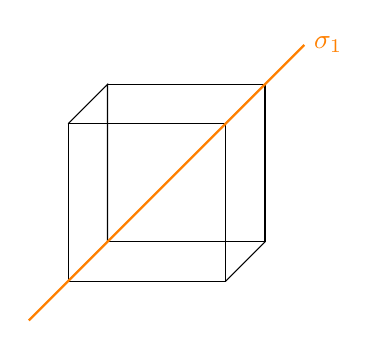
\begin{tikzpicture}[baseline=(current bounding box.south)]
                    % Coordinates of the vertices
                    \coordinate (A) at (0, 0);
                    \coordinate (B) at (0, 2);
                    \coordinate (C) at (2, 2);
                    \coordinate (D) at (2, 0);
                    \coordinate (E) at (0.5, 0.5);
                    \coordinate (F) at (0.5, 2.5);
                    \coordinate (G) at (2.5, 2.5);
                    \coordinate (H) at (2.5, 0.5);

                    % The cube
                    \draw (A) -- (B) -- (C) -- (D) -- cycle;
                    \draw (A) -- (E) -- (F) -- (B);
                    \draw (D) -- (H) -- (G) -- (C);
                    \draw (E) -- (F) -- (G) -- (H) -- cycle;

                    % The plane
                    \draw[thick,orange] (-0.5, -0.5) -- (3, 3);
                    \node[orange,right] at (3, 3) {$\sigma_1$};
                \end{tikzpicture}
                \hfil%
                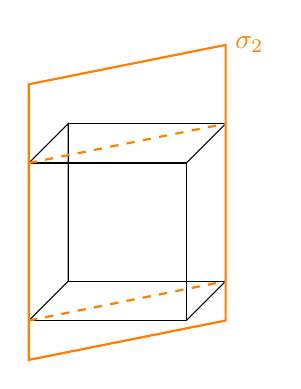
\begin{tikzpicture}[baseline=(current bounding box.south)]
                    % Coordinates of the vertices
                    \coordinate (A) at (0, 0);
                    \coordinate (B) at (0, 2);
                    \coordinate (C) at (2, 2);
                    \coordinate (D) at (2, 0);
                    \coordinate (E) at (0.5, 0.5);
                    \coordinate (F) at (0.5, 2.5);
                    \coordinate (G) at (2.5, 2.5);
                    \coordinate (H) at (2.5, 0.5);

                    % The cube
                    \draw (A) -- (B) -- (C) -- (D) -- cycle;
                    \draw (A) -- (E) -- (F) -- (B);
                    \draw (D) -- (H) -- (G) -- (C);
                    \draw (E) -- (F) -- (G) -- (H) -- cycle;

                    % The plane
                    \draw[thick,orange] (0, -0.5) -- (0, 3) -- (2.5, 3.5) -- (2.5, 0) -- cycle;
                    \draw[thick,dashed,orange] (A) -- (H);
                    \draw[thick,dashed,orange] (B) -- (G);
                    \node[orange,right] at (2.5, 3.5) {$\sigma_2$};
                \end{tikzpicture}
                \hfil
                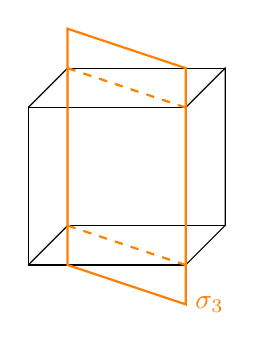
\begin{tikzpicture}[baseline=(current bounding box.south)]
                    % Coordinates of the vertices
                    \coordinate (A) at (0, 0);
                    \coordinate (B) at (0, 2);
                    \coordinate (C) at (2, 2);
                    \coordinate (D) at (2, 0);
                    \coordinate (E) at (0.5, 0.5);
                    \coordinate (F) at (0.5, 2.5);
                    \coordinate (G) at (2.5, 2.5);
                    \coordinate (H) at (2.5, 0.5);

                    % The cube
                    \draw (A) -- (B) -- (C) -- (D) -- cycle;
                    \draw (A) -- (E) -- (F) -- (B);
                    \draw (D) -- (H) -- (G) -- (C);
                    \draw (E) -- (F) -- (G) -- (H) -- cycle;

                    % The plane
                    \draw[thick,orange] (0.5, 3) -- (2, 2.5) -- (2, -0.5) -- (0.5, 0) -- cycle;
                    \draw[thick,dashed,orange] (C) -- (F);
                    \draw[thick,dashed,orange] (D) -- (E);
                    \node[orange,right] at (2, -0.5) {$\sigma_3$};
                \end{tikzpicture}
            \end{center}

            % TODO: graphs of $\sigma_1$, $\sigma_2$, and $\sigma_3$. 
    \end{remark}

    \begin{center}
        \begin{tikzpicture}
            % The cube expanded to 2D
            \draw (0, 0) -- (0, 2) -- (2, 2) -- (2, 0) -- cycle;
            \draw (0, 0) -- (-2, 0) -- (-2, 2) -- (0, 2);
            \draw (2, 2) -- (4, 2) -- (4, 0) -- (2, 0);
            \draw (4, 2) -- (6, 2) -- (6, 0) -- (4, 0);
            \draw (0, 2) -- (0, 4) -- (2, 4) -- (2, 2);
            \draw (2, 0) -- (2, -2) -- (0, -2) -- (0, 0);

            % Crosses on the cube
            \draw[dashed] (-2, 2) -- (0, 0) -- (2, 2) -- (4, 0) -- (6, 2);
            \draw[dashed] (-2, 0) -- (0, 2) -- (2, 0) -- (4, 2) -- (6, 0);
            \draw[dashed] (0, 4) -- (2, 2);
            \draw[dashed] (0, 2) -- (2, 4);
            \draw[dashed] (0, -2) -- (2, 0);
            \draw[dashed] (0, 0) -- (2, -2);

            % The vertices
            \node[graph-node,blue]   at (-2, 0) {};
            \node[graph-node,orange] at (-2, 2) {};
            \node[graph-node,orange] at (0, 0) {};
            \node[graph-node,blue]   at (0, 2) {};
            \node[graph-node,orange] at (2, 2) {};
            \node[graph-node,blue]   at (2, 0) {};
            \node[graph-node,orange] at (0, 2) {};
            \node[graph-node,blue]   at (2, 2) {};
            \node[graph-node,orange] at (2, -2) {};
            \node[graph-node,blue]   at (0, -2) {};
            \node[graph-node,blue]   at (4, 2) {};
            \node[graph-node,orange] at (4, 0) {};
            \node[graph-node,orange] at (6, 2) {};
            \node[graph-node,blue]   at (6, 0) {};

            % The centers of the crosses
            \node[graph-node,red] at (-1, 1) {};
            \node[graph-node,red] at (1, 1) {};
            \node[graph-node,red] at (1, 1) {};
            \node[graph-node,red] at (1, 3) {};
            \node[graph-node,red] at (1, -1) {};
            \node[graph-node,red] at (3, 1) {};
            \node[graph-node,red] at (5, 1) {};

            % The label $C$
            \node[magenta] at (1.5, 1) {$C$};
            \node[magenta] at (2.5, 1) {$\sigma_1C$};
            \node[magenta] at (1, 1.5) {$\sigma_2C$};
            \node[magenta] at (1, 0.5) {$\sigma_3C$};
            \node[magenta] at (0.5, 1) {$D$};
        \end{tikzpicture}
    \end{center}

    $D$ can be obtained by either $\sigma_3 \sigma_2 C$ or $\sigma_2 \sigma_3 C$. \[ \begin{matrix}
        \mathbb{R}^3 & \to & \mathbb{R}^3 & \to & \mathbb{R}^3 \\
        & \sigma_3 & & \sigma_2 & \\
        & \sigma_2 & & \sigma_3 &
    \end{matrix} \]

    Matrices are not commute, and thus these transformations may be different. We ask the questions: since $\sigma_2 \sigma_1$ and $\sigma_1 \sigma_2$ move the triangle $C$ in the same way, are they the same map?

    \begin{proposition}
        If $S, T: \mathbb{R}^3 \to \mathbb{R}^3$ preserve the coloured ube and send the triangle to the same place, then $S = T$ (as maps). 
    \end{proposition}

    \begin{proof}
        WTS $S = T$.

        \begin{remark}
            It is important that the triangle $C$ is a field of vectors. 
        \end{remark}
        Consider $o = (0, 0, \frac{1}{2})$, $b = (\frac{1}{2}, \frac{1}{2}, \frac{1}{2})$, and $y = (-\frac{1}{2}, \frac{-1}{2}, \frac{1}{2})$. 

        $Sb = Tb, So = To, Sy = Ty \implies (S - T)b = 0, (S - T)o = 0, (S - T)y = 0$.

        This implies $b$, $o$, and $y$ are in the kernel of $S - T$. 

        Moreover, $b, o, y$ are linearly independent since $\det \begin{bmatrix}
            \frac{1}{2} & 0 & -\frac{1}{2} \\
            \frac{1}{2} & 0 & -\frac{1}{2} \\
            \frac{1}{2} & \frac{1}{2} & \frac{1}{2}
        \end{bmatrix} \neq 0$.

        Thus, $\dim \ker (S - T) = 3$. Since $\dim \mathbb{R}^3 = 3$, $\ker (S - T) = \mathbb{R}^3$. Thus, $S - T = 0$.
    \end{proof}

    We can reach all 24 locations of the triangle $C$ by applying $\sigma_1$, $\sigma_2$, and $\sigma_3$ to the triangle $C$. Thus, there are 24 isometries that preserve the coloured cube. Moreover, we know that $3$ of them generates the set. It suffices to study these three isometries to understand the whole group.
\end{example}
\chapter{Introduction to Group}

\section{Introduction}

\begin{remark}
    What have we done so far: we have studied some \bred{objects} with some properties, and we have asked how can we operate in this object and preserve its property. 
\end{remark}

\begin{definition}[Group]\index{Group}\label{def:group}
    A \term{group} is a pair $(G, \cdot)$ where $G$ is a set and $\cdot$ is a binary operation on $G$ such that \[
        \begin{matrix}[cccc]
            \cdot & G \times G & \to     & G         \\
                  & (a, b)     & \mapsto & a \cdot b
        \end{matrix}
    \] such that \begin{listu}
        \item \textbf{Identity:} There exists an element $e \in G$ such that \[ e \cdot g = g \cdot e = a \quad \forall a \in G. \]
        \item \textbf{Inverse:} For every $g \in G$ there exists an element $h \in G$ such that \[ g \cdot h = h \cdot g = e. \]
        \item \textbf{Associativity:} For every $g, h, k \in G$ we have \[ g \cdot (h \cdot k) = (g \cdot h) \cdot k. \]
    \end{listu}
\end{definition}

\begin{definition}[Abelian Group]\index{Abelian Group}\label{def:abelian_group}
    A group $(G, \cdot)$ is called \term{abelian} if \[ g \cdot h = h \cdot g \quad \forall g, h \in G. \]

    This group is also called a \term{commutative group}.
\end{definition}

The term \textit{abelian} comes from the name of the Norwegian mathematician \href{https://en.wikipedia.org/wiki/Niels_Henrik_Abel}{Niels Henrik Abel}. He was the first to prove the impossibility of solving the general quintic equation in radicals. He also made important contributions to the study of elliptic functions, discovered Abelian functions, and many other important fields in mathematics.

\begin{example}
    We will consider the following ``toy"

    \begin{center}
        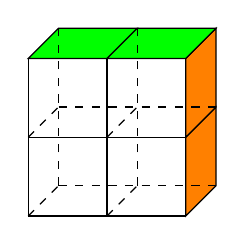
\begin{tikzpicture}
            \draw (0,0,0) -- (1,0,0) -- (1,1,0) -- (0,1,0) -- cycle;
            \draw (1,0,0) -- (2,0,0) -- (2,1,0) -- (1,1,0) -- cycle;
            \draw (0,1,0) -- (1,1,0) -- (1,2,0) -- (0,2,0) -- cycle;
            \draw (1,1,0) -- (2,1,0) -- (2,2,0) -- (1,2,0) -- cycle;

            \draw[fill=orange] (2,0,0) -- (2,0,-1) -- (2,1,-1) -- (2,1,0) -- cycle;
            \draw[fill=orange] (2,1,0) -- (2,1,-1) -- (2,2,-1) -- (2,2,0) -- cycle;

            \draw[fill=green] (0,2,0) -- (1,2,0) -- (1,2,-1) -- (0,2,-1) -- cycle;
            \draw[fill=green] (1,2,0) -- (2,2,0) -- (2,2,-1) -- (1,2,-1) -- cycle;

            % Dashed invisible lines
            \draw[dashed] (0,0,0) -- (0,0,-1);
            \draw[dashed] (1,0,0) -- (1,0,-1);
            \draw[dashed] (0,1,0) -- (0,1,-1);
            \draw[dashed] (1,1,0) -- (1,1,-1);
            \draw[dashed] (0,0,-1) -- (0,2,-1);
            \draw[dashed] (1,0,-1) -- (1,2,-1);
            \draw[dashed] (0,0,-1) -- (2,0,-1);
            \draw[dashed] (0,1,-1) -- (2,1,-1);
        \end{tikzpicture}

        The left side is red, the bottom is blue, and the back is yellow. 
    \end{center}

    We have $7$ operations \[
        V_1, V_2, H_1, H_2, V, H, R
    \] where \begin{listu}
        % TODO: add picture
        \item $V_1$ is the vertical flip of the first column
        \item $V_2$ is the vertical flip of the second column
        \item $H_1$ is the horizontal flip of the first row
        \item $H_2$ is the horizontal flip of the second row
        \item $V$ is the vertical flip of the whole cube
        \item $H$ is the horizontal flip of the whole cube
        \item $R$ is the rotation of the cube by $90^\circ$ around the vertical axis
    \end{listu}
    
    They satisfy \[
        {V_1}^2 = 1, {V_2}^2 = 1, {H_1}^2 = 1, {H_2}^2 = 1, V^2 = 1, H^2 = 1, R^4 = 1, 
    \]

    However, we have redundancies: \begin{listu}
        \item $V_1 V_2 = V_2 V_1 = V$
        \item $H_1 H_2 = H_2 H_1 = H$
        \item $V_1 H_1 = H_1 V_1 = R$
        \item $H_2 H_1 V_2 V_1 = R^2$
        \item $R^3 V_1 R = R^{-1} V_1 R = H_1$ 
        \item \dots
    \end{listu}

    We can flatten the cube into
    \begin{center} \begin{tabular}{c|c} 1 & 2 \\ \hline 3 & 4 \end{tabular} \end{center}

    Then, \begin{listu}
        \item $V_1 = (1, 4)$ 
        \begin{center} 
            \begin{tabular}{c|c} 1 & 2 \\ \hline 4 & 3 \end{tabular}
            \quad$\xrightarrow{V_1}$\quad
            \begin{tabular}{c|c} 4 & 2 \\ \hline 1 & 3 \end{tabular} 
        \end{center}

        \item $V_2 = (2, 3)$
        \begin{center} 
            \begin{tabular}{c|c} 1 & 2 \\ \hline 4 & 3 \end{tabular}
            \quad$\xrightarrow{V_2}$\quad
            \begin{tabular}{c|c} 1 & 3 \\ \hline 4 & 2 \end{tabular}
        \end{center}

        \item $H_1 = (1, 2)$
        \begin{center} 
            \begin{tabular}{c|c} 1 & 2 \\ \hline 4 & 3 \end{tabular}
            \quad$\xrightarrow{H_1}$\quad
            \begin{tabular}{c|c} 4 & 3 \\ \hline 1 & 2 \end{tabular}
        \end{center}

        \item $H_2 = (3, 4)$
        \begin{center} 
            \begin{tabular}{c|c} 1 & 2 \\ \hline 4 & 3 \end{tabular}
            \quad$\xrightarrow{H_2}$\quad
            \begin{tabular}{c|c} 1 & 2 \\ \hline 3 & 4 \end{tabular}
        \end{center}

        % \item $V = (1, 4)(2, 3)$

        \item $R = (1, 2, 3, 4)$
        \begin{center} 
            \begin{tabular}{c|c} 1 & 2 \\ \hline 4 & 3 \end{tabular}
            \quad$\xrightarrow{R}$\quad
            \begin{tabular}{c|c} 4 & 1 \\ \hline 3 & 2 \end{tabular}
        \end{center}
    \end{listu}

    We can verify that \[
        (1, 2, 3, 4) = (3, 4)(1, 4)(1, 2),
    \] which proposes that \[
        R = H_2 \circ V_1 \circ H_1
    \]

    % TODO: add picture
\end{example}

We have a group that is the one generator by the operations of the `toy` above. We have two models to understand the group: \begin{listo}
    \item The complete toy 
    \item The location code
\end{listo} What we have seen is that these two models are codify information in different ways. We can generate a map of the potential positions. 

% TODO: image

\begin{center}
    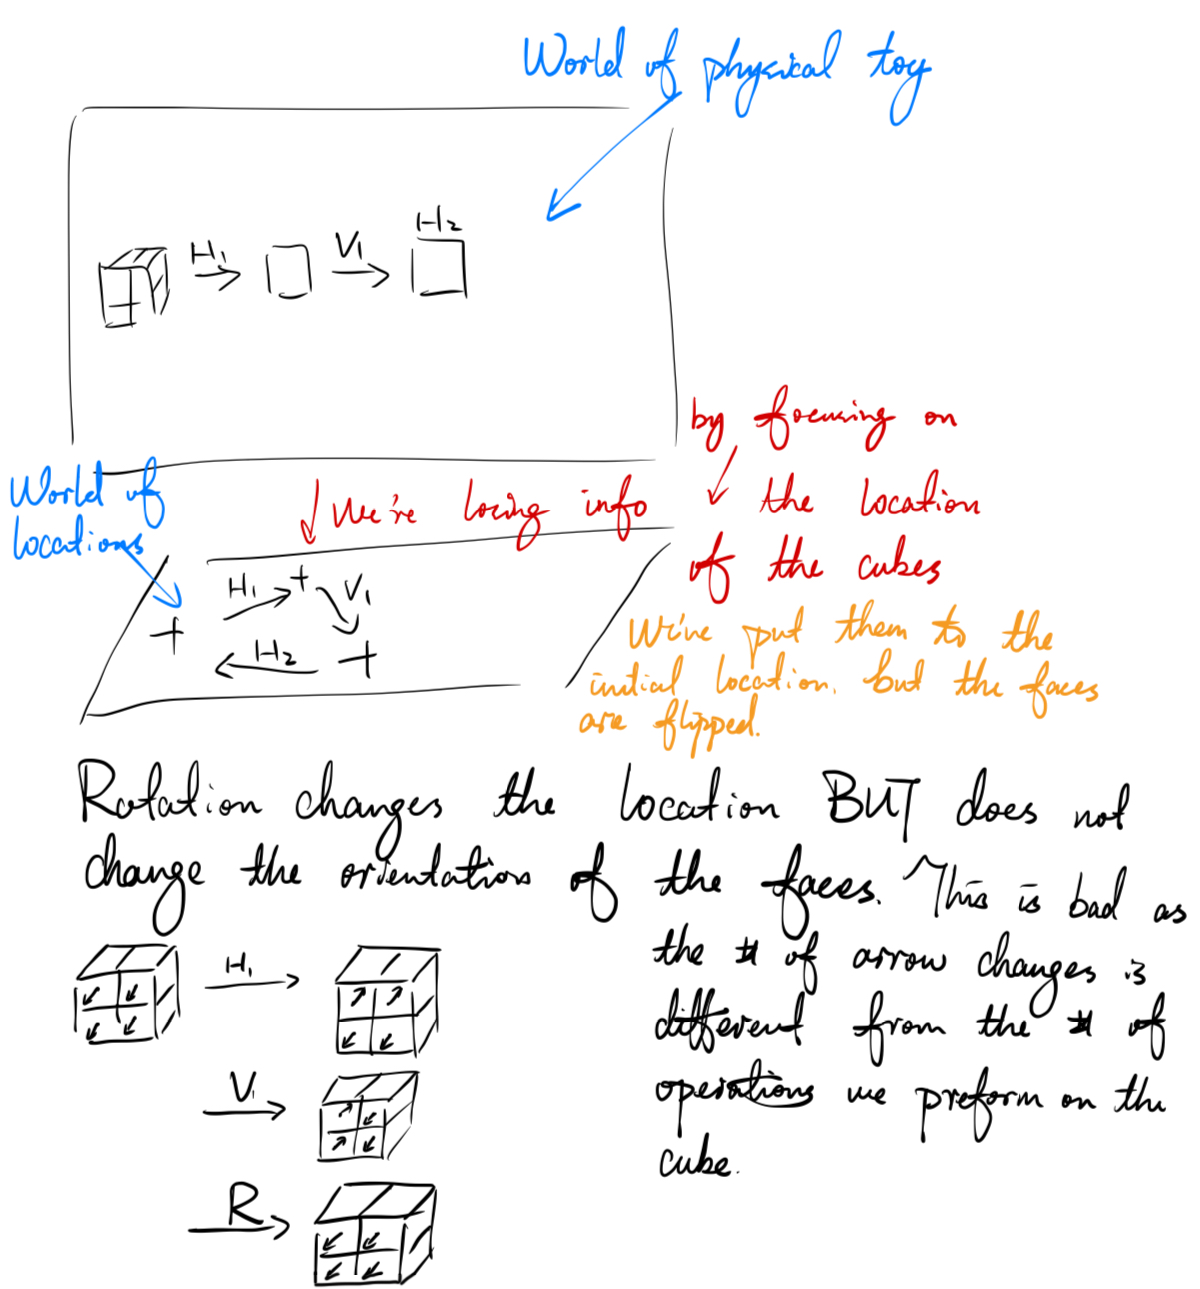
\includegraphics[width=0.55\linewidth]{figures/rubics-cube-1.png}
\end{center}

If we only allow $H_1, V_1, H_2, V_2$, then the locations are believable. The group they generate is $S_4$. 

\begin{remark}
    Think of $S_4$ independently. 

    We consider the permutations independently as a group. 

    \begin{center}
        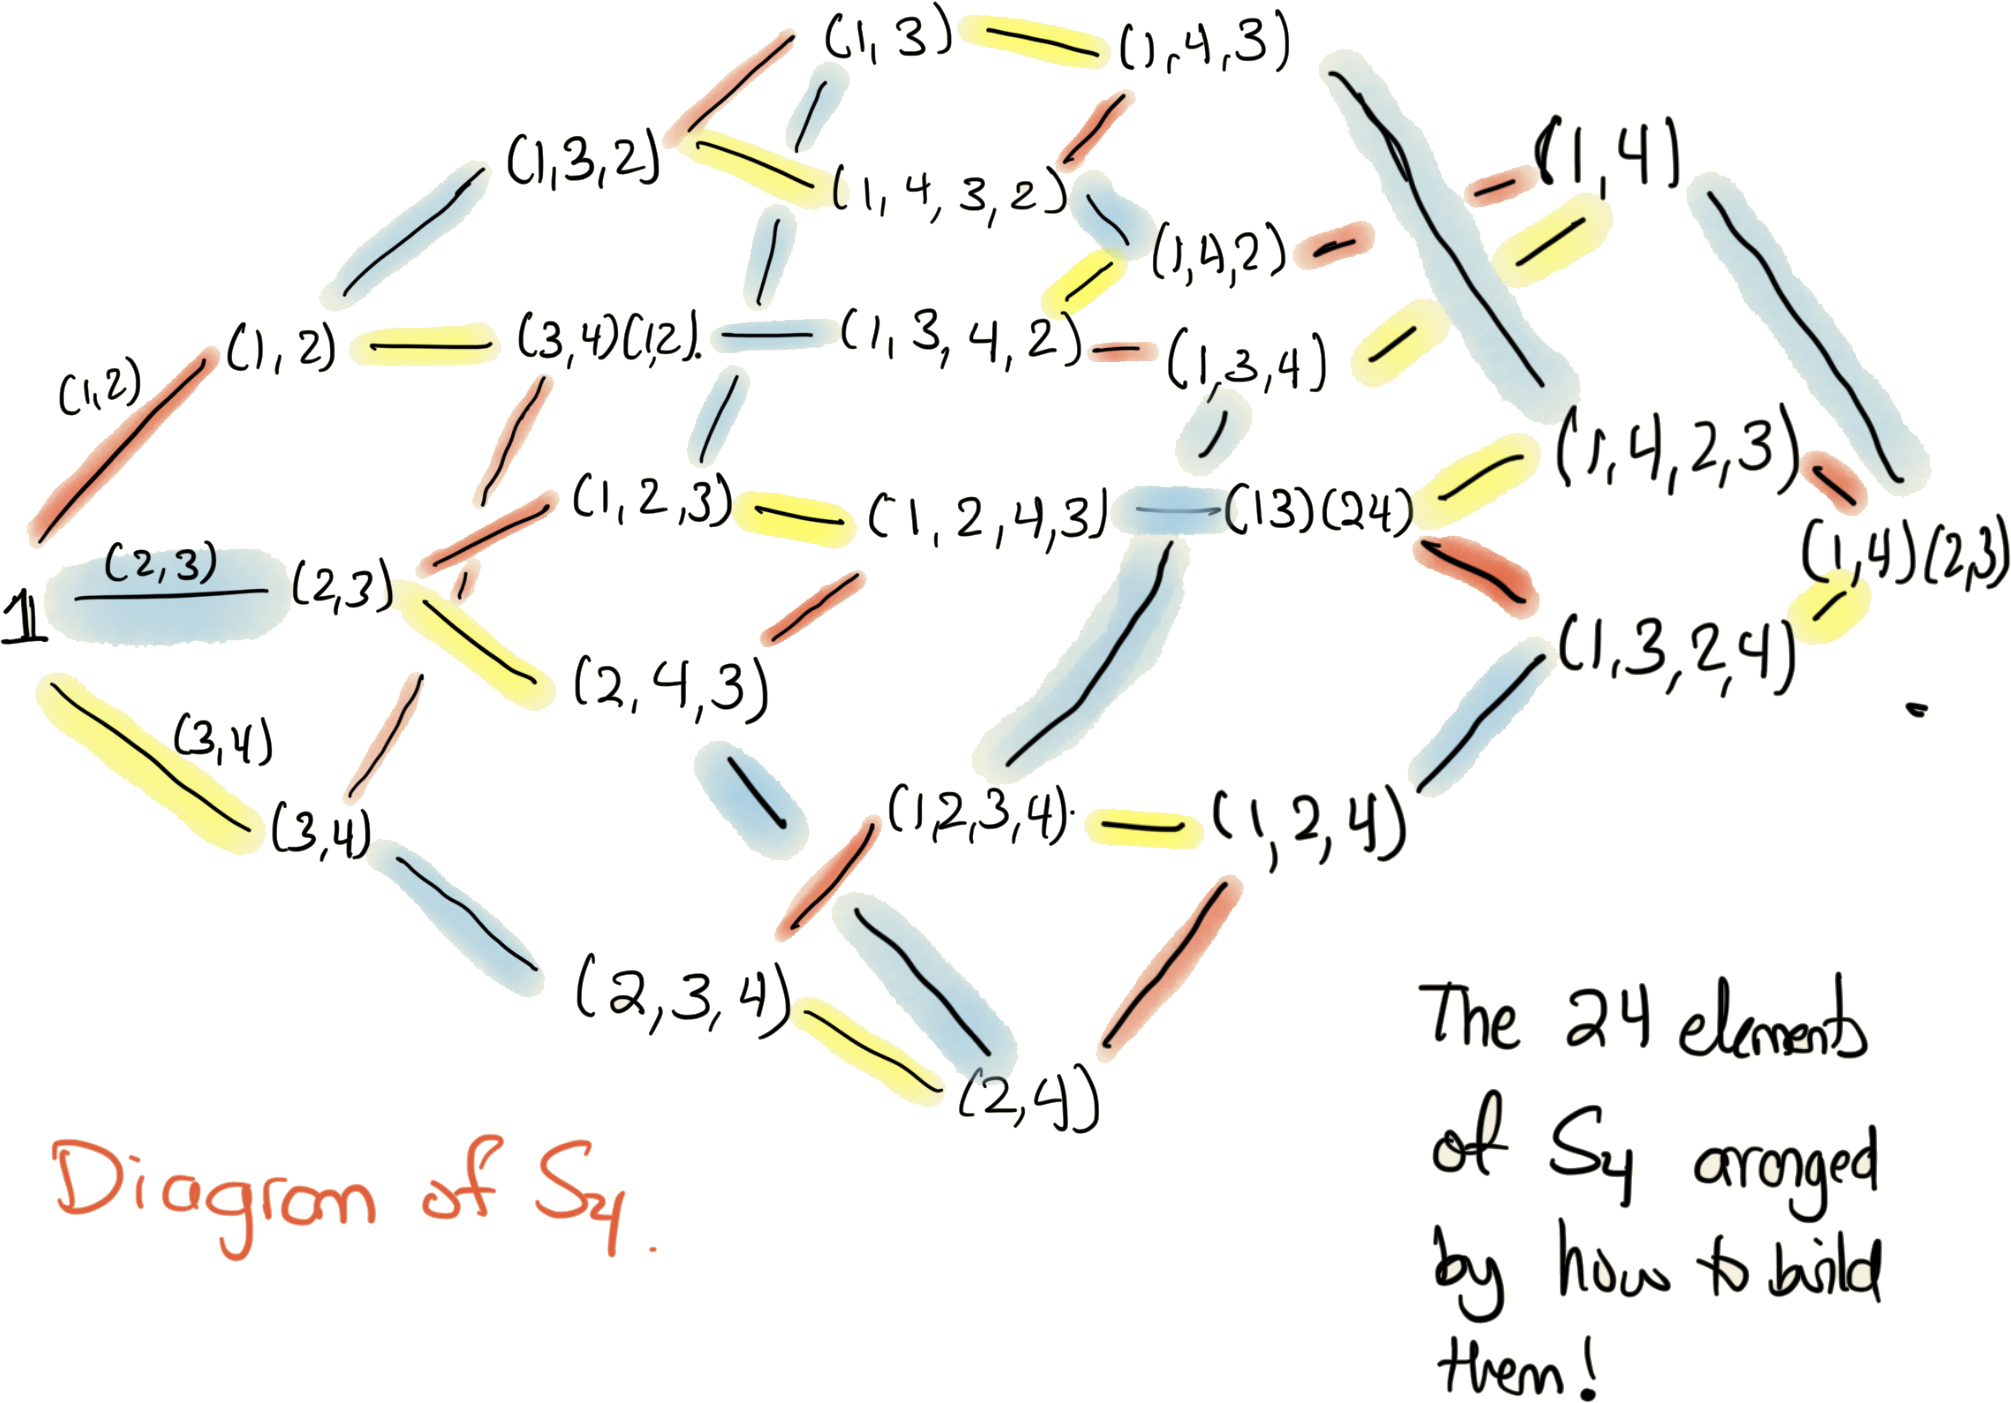
\includegraphics[width=0.55\linewidth]{figures/permutations-of-s4.png}
    \end{center}
\end{remark}

We want to merge $R$ with the rest of the operations. 

Consider \[
    H_1 R = R V_1 \qquad H_2 R = R V_2
\]

\begin{center}
    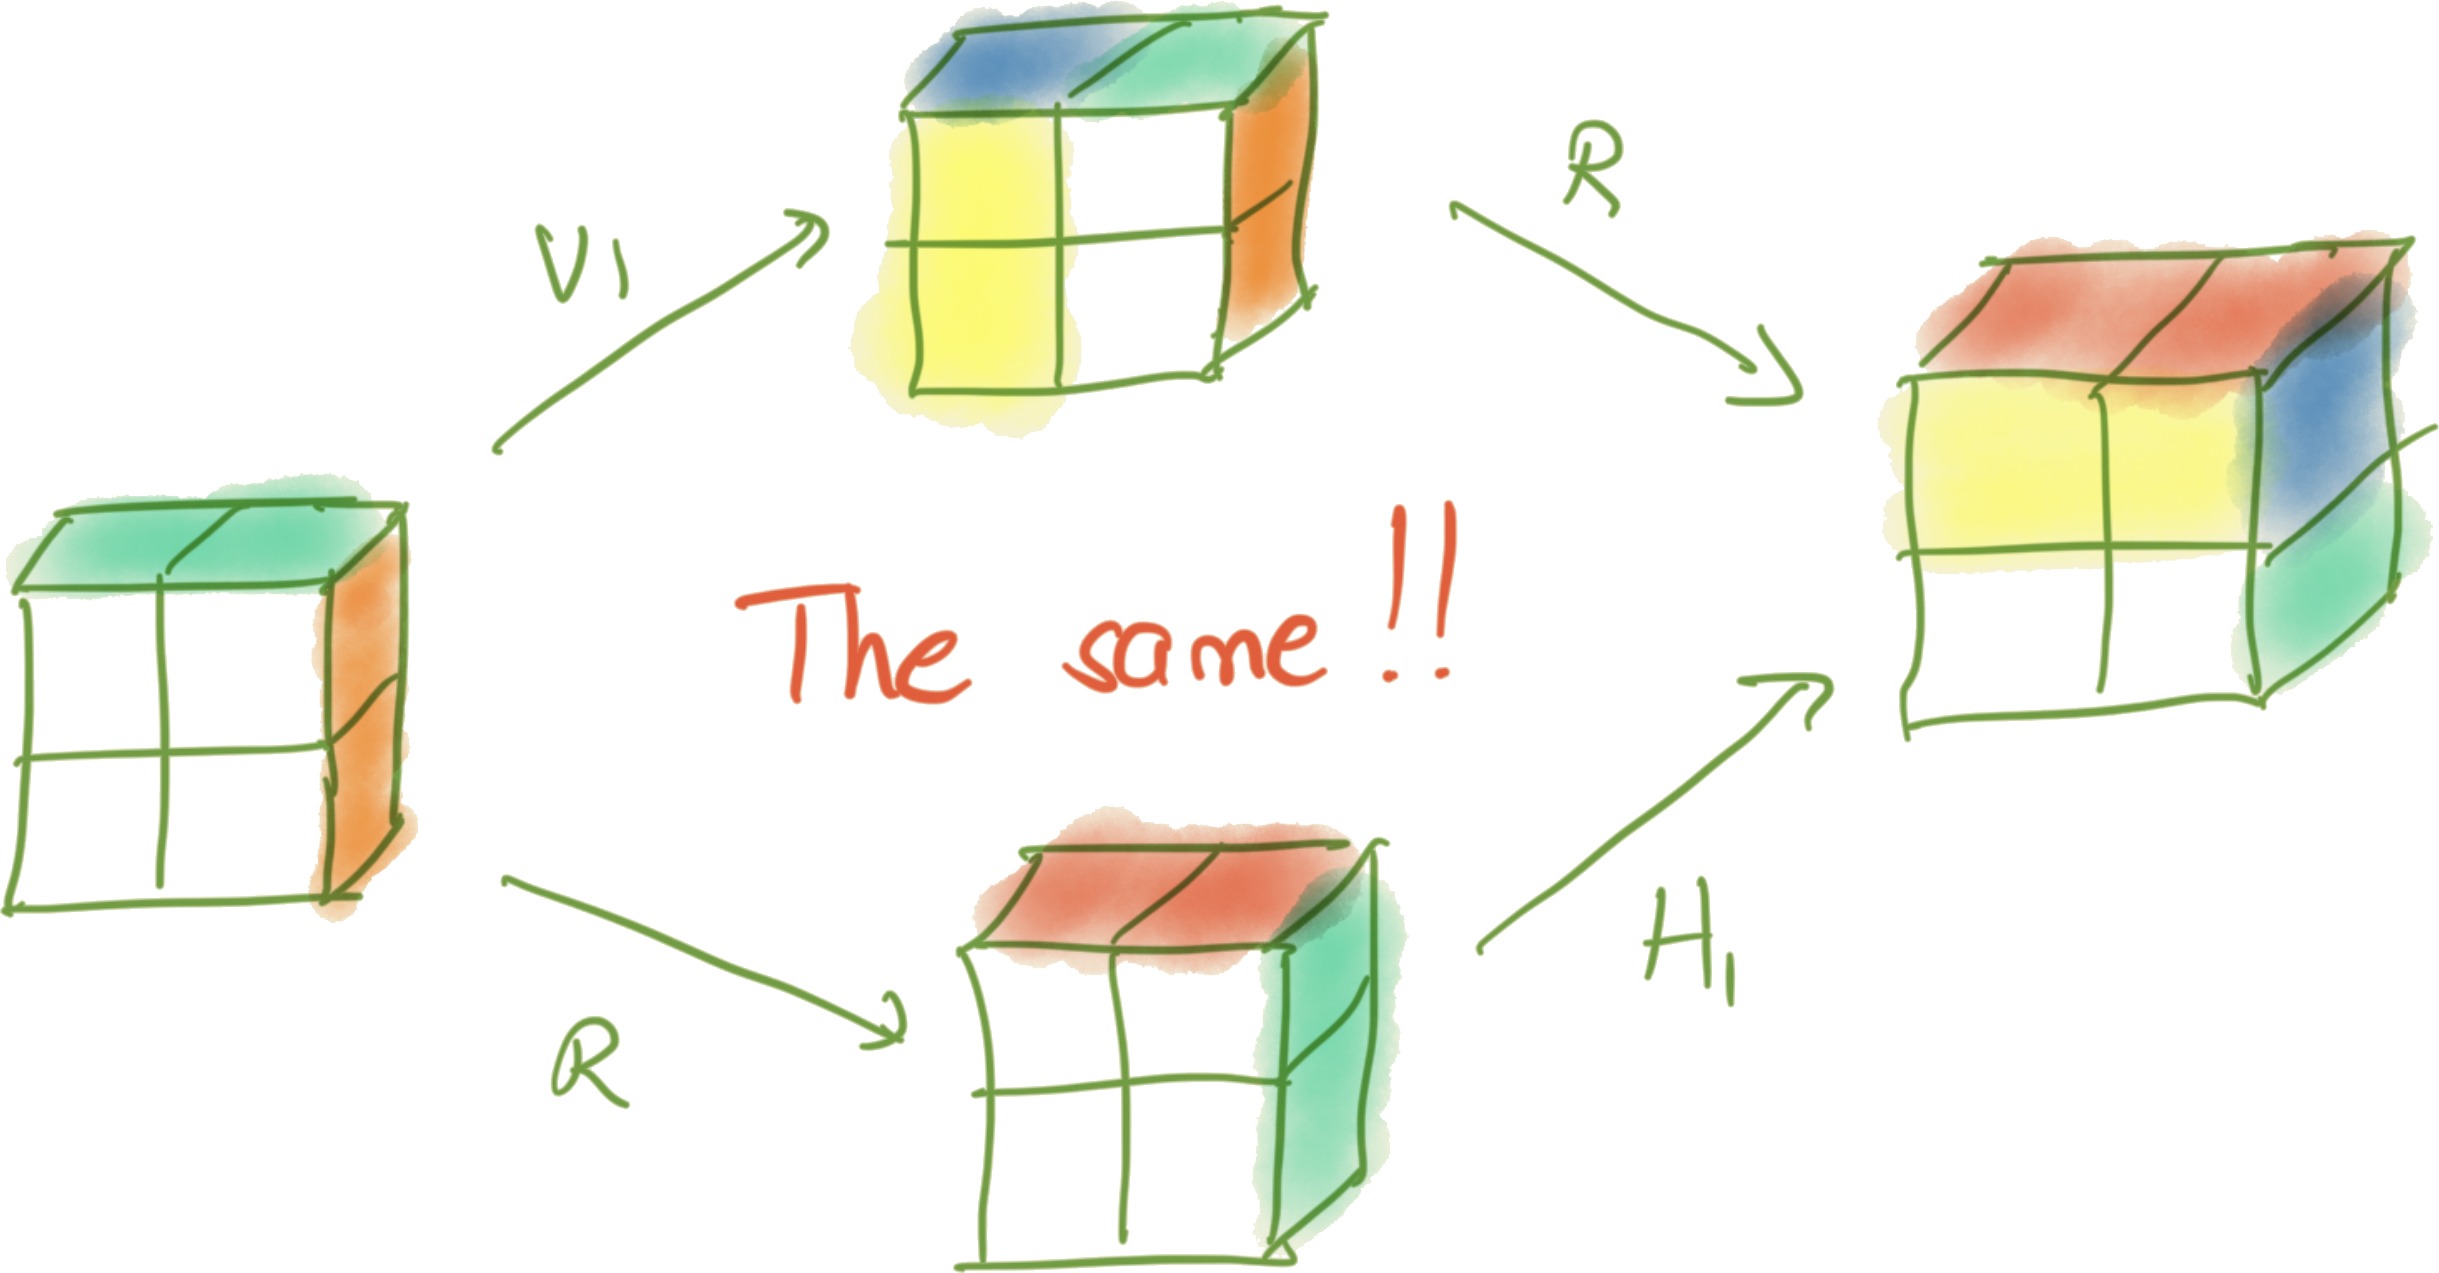
\includegraphics[width=0.45\linewidth]{figures/r-v1.png}
\end{center}

\begin{example}
    ``Simplify'' the instructions  \[
        R V_1 H_2 R V_2 H_1 H_2 R V_1 H_2
    \]

    Using the two equations above, 
    \begin{align*}
        R V_1 H_2 R V_2 H_1 H_2 R V_1 H_2
         & = R V_1 H_2 R V_2 H_1 {\color{red}R V_2} V_1 H_2             \\
         & = R V_1 H_2 R V_2 {\color{red}R V_1} V_2 V_1 H_2             \\
         & = R V_1 H_2 R {\color{red}R H_2} V_1 V_2 V_1 H_2             \\
         & = R V_1 H_2 {\color{red}V_1 V_2 H_1 H_2} H_2 V_1 V_2 V_1 H_2
         & (RR = V_1 V_2 H_1 H_2)                                       \\
    \end{align*}

    This way, we have moved all the ``noice'', $R$, to the last steps. 
\end{example}

\textbf{Fact:} All elements of the group can be written as \[
    X \sigma
\] where $X = 1 \text{ or } R$ and $\sigma \in S_4$. 

\begin{proposition}
    This writing is \bred{unique}. 
\end{proposition}

\begin{proof}
    Suppose $X_1 \sigma_1 = X_2 \sigma_2$. 

    \begin{listu}
        \item If $X_1 = X_2 = 1$, then $\sigma_1 = \sigma_2$.

        \item If $X_1 = X_2 = R$, then $R \sigma_1 = R \sigma_2$.

        Multiplying by $R^{-1}$, we have \[ \begin{aligned}[t]
            R^{-1} R \sigma_1 & = R^{-1} R \sigma_2 \\
            \sigma_1          & = \sigma_2
        \end{aligned} \]

        \item $X_1 = 1, X_2 = R$. Then, \[ \begin{aligned}[t]
            \sigma_1 & = R \sigma_2 \\
            \sigma_1 {\sigma_2}^{-1} & = R \sigma_2 {\sigma_2}^{-1} \\
            \sigma_1 {\sigma_2}^{-1} & = R
        \end{aligned} \] which means $R \in S_4$, which is impossible.
    \end{listu}
\end{proof}

These decomposition also has coordinates. $X$ uses the $R$-coordinate and $\sigma$ uses the $S_4$-coordinate.

We can write this as \[
    (1, \sigma) \in \pm 1 \times S_4
\]

However, note that $(s_1, \sigma_1) (s_2, \sigma_2) = (s_1 s_2, \sigma_1 \sigma_2)$ is \bred{not true}. The reason is because there is ``noice'' (procued by $R$) in the first coordinate.

\begin{center}
    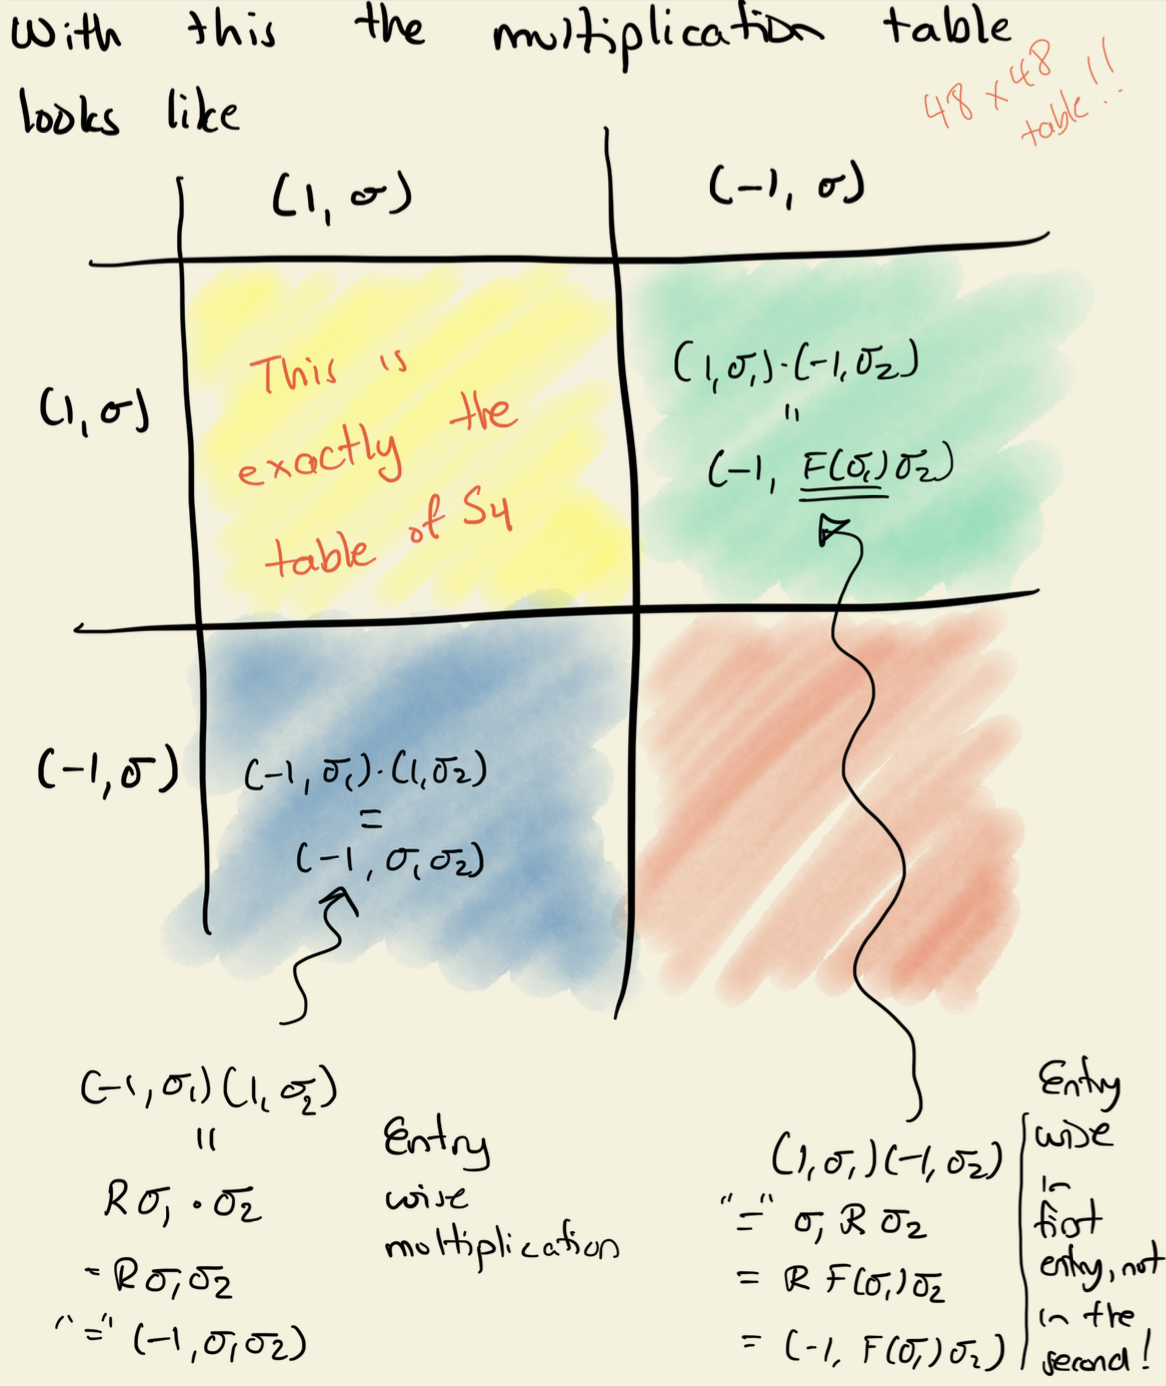
\includegraphics[width=0.67\linewidth]{figures/rotation_s4_table.png}
\end{center}
\chapter{Cyclic Groups}

\section{Introduction}

For every positive integer $n$, we consider the integers modulo $n$. 

\begin{example}
    For $n = 3$, we have the multiplication table:

    \begin{minipage}[h]{0.45\linewidth} \begin{center}
        \begin{tabular}{c|c|c|c}
            $+$ & 0 & 1 & 2 \\ \hline
            0   & 0 & 1 & 2 \\ \hline
            1   & 1 & 2 & 0 \\ \hline
            2   & 2 & 0 & 1
        \end{tabular}
    \end{center} \end{minipage}
    \begin{minipage}[h]{0.45\linewidth} \begin{center}
        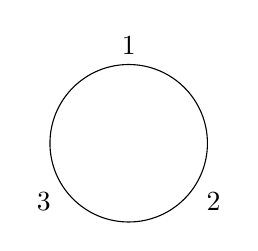
\begin{tikzpicture}
            \draw (0, 0) circle (1);
            
            \node[above] (1) at (0, 1) {1};
            \node[below right] (2) at (0.866, -0.5) {2};
            \node[below left] (3) at (-0.866, -0.5) {3};

            % Arc from 1 to 2, 2 to 3, 3 to 1, with text $+1$ on each arc
            % TODO
        \end{tikzpicture}
    \end{center} \end{minipage}

    Similarly, for $n = 4$, we have the multiplication table:

    \begin{table}[ht!]
        \centering
        \begin{tabular}{c|c|c|c|c}
            $+$ & 0 & 1 & 2 & 3 \\ \hline
            0   & 0 & 1 & 2 & 3 \\ \hline
            1   & 1 & 2 & 3 & 0 \\ \hline
            2   & 2 & 3 & 0 & 1 \\ \hline
            3   & 3 & 0 & 1 & 2
        \end{tabular}
    \end{table}
\end{example}

\begin{definition}[Cuclic Group]\index{Cyclic Group}\label{def:cyclic-group}
    Let $n$ be a positive integer. A \term{cyclic group} of order $n$ is one that admits a generator of order $n$. \[
        C_n = \{ 0, 1, \dots, n - 1 \}
    \]
\end{definition}

\begin{definition}[Generator]\index{Generator}\label{def:generator}
    A \term{generator} of a group $G$ is an element $g \in G$ such that every element of $G$ can be written as a power of $g$.
\end{definition}

The group of integers modulo $n$ is called the \term{cyclic group of order $n$} and is denoted by $C_n$ or $\Z/n\Z$.

\begin{example}
    The integers $\Z$ form a cyclic group under addition. \[ 
        \cdots \xrightarrow{+1} -2 \xrightarrow{+1} -1 \xrightarrow{+1} 0 \xrightarrow{+1} 1 \xrightarrow{+1} 2 \xrightarrow{+1} \cdots 
    \]
\end{example}

Given a group $G$ and an element $g \in G$, we produce \[
    \underbrace{\left\{ \dots, g^{-2}, g^{-1}, 1 = g^0, g, g^2, g^3, \dots \right\}}_{\langle g \rangle} \subseteq G
\]

\begin{proposition}\label{prop:order-of-cyclic-group}
    Let $G$ be a group and $g \in G$. 

    \begin{listo}
        \item The set of powers of $g$, \[
            \left\{ g^m \mid m \in \Z \right\}
        \] is a subgroup of $G$ (denoted by $\langle g \rangle$).

        \item $g$ has order $m$ if and only if $\langle g \rangle$ is isomorphic to $C_m$.
        
        \item $g$ has no order if and only if $\langle g \rangle$ is isomorphic to $\Z$.
    \end{listo}
\end{proposition}

\begin{proof}(Proposition \ref{prop:order-of-cyclic-group}.1)
    WTS $\langle g \rangle$ is a subgroup of $G$.

    \begin{listu}
        \item \textbf{Associativity} follows from that of $G$. 

        \item \textbf{Identity} is a power of $g$, namely, $g^0 = 1$.

        \item Each element has an \textbf{inverse}, indeed, the inverse of $g^n$ is $g^{-n}$ which is also a power. 

        \item \textbf{Closed} under the operation \[
            g^n \cdot g^m = g^{n + m}
        \] which is also a power. 
    \end{listu}
\end{proof}

\begin{proof}(Proposition \ref{prop:order-of-cyclic-group}.2)
    WTS $g$ has order $m$ if and only if $\langle g \rangle \cong C_m$.

    If $G$ has order $m$, \[
        1, g, g^2, \dots, g^{m - 1}
    \] are distinct.

    Define $\Phi: C_m \to \langle g \rangle$ by $\Phi(k) = g^k$.

    This is well defined if $a \equiv b \pmod{m}$, then $a = b + mt$ for some $t \in \Z$. \[
        g^a = g^{b + mt} = g^b \cdot g^{mt} = g^b \cdot (g^m)^t = g^b \cdot 1^t = g^b
    \] 

    It is an homomorphism, indeed, \[
        \Phi(a + b) = g^{a + b} = g^a \cdot g^b = \Phi(a) \cdot \Phi(b)
    \]

    \begin{listu}
        \item \textbf{Injectivity}
        
        If $\Phi(a) = \Phi(b)$, then $g^a = g^b$, so $g^{a - b} = 1$.

        We can pick $a, b \in \{ 0, 1, \dots, m - 1 \}$. We can also suppose $a \ge b$, thus \[
            0 \le a - b \le m - 1
        \]

        Then $g^{a - b} = 1$ implies $a - b = 0$, for owtherwise $g$ has order smaller than $m$. 

        Thus, $a = b$, so $\Phi$ is injective.

        \item \textbf{Surjectivity}

        By assumption \[
            \langle h \rangle = \{ g^0, g^1, \dots, g^{m - 1} \}
        \]

        Since by definition \[
            \Phi(k) = g^k,
        \] by taking $k = 0, 1, \dots, m - 1$ we produce all elements of $\langle g \rangle$.

        Thus, $\Phi$ is surjective.
    \end{listu}

    We conclude that $\Phi$ is an isomorphism.
\end{proof}

\begin{example}
    Consider $C_6 = \{ 0, 1, 2, 3, 4, 5 \}$.

    The cyclic groups the elements generate are
    \begin{listu}
        \item $0$ generates $\{ 0 \} \equiv C_1$.
        \item $1$ and $5$ generate $\equiv C_6$, $C_6 = \langle 1 \rangle = \langle 5 \rangle$.
        \item $\langle 2 \rangle = \{ 0, 2, 4\} = \langle 4 \rangle \cong C_3$. 
        \item $\langle 3 \rangle = \{ 0, 3 \} \cong C_2$.
    \end{listu}
\end{example}

\begin{example}
    We have already seen in a previous example what happens. The cyclic subgroups are

    \begin{listu}
        \item $\langle 1 \rangle = \{ \id \} = C_1$.
        \item $\langle (1, 2) \rangle = \{ \id, \langle (1, 2) \rangle \} = C_2$
        \item $\langle (1, 3) \rangle = \{ \id, \langle (1, 3) \rangle \} = C_2$
        \item $\langle (2, 3) \rangle = \{ \id, \langle (2, 3) \rangle \} = C_2$
        \item $\langle (1, 2, 3) \rangle = \{ \id, (1, 2, 3), (1, 3, 2) \rangle \} = C_3$
    \end{listu}
\end{example}

\begin{proposition}
    Let $p$ be a prime number, and $G$ be a group of order $p$. Then $G$ is cyclic, \[
        G \cong C_p
    \]
\end{proposition}

\begin{proof}
    Let $G$ be a group of order $p$. 
    
    Since $p$ is prime, $G$ has at least two elements. Thus, there exists $g \in G$ with $g \neq e$. 

    Since $G$ is finite, $g$ must have a finite order $m$. Thus, \[
        C_m = \{ 1, g, g^2, \dots, g^{m - 1} \} \subseteq G
    \]

    Let $x \in G$ and multiply by $g$ successively by the left. \[
        x \xrightarrow{g} gx \xrightarrow{g} g^2x \xrightarrow{g} \cdots \xrightarrow{g} g^{m - 1}x \xrightarrow{g} g^mx = x
    \]

    There is no repetition earlier than $m$, since otherwise $g^ix = g^jx$ for some $0 \le i < j \le m - 1$, so $g^i = g^j$ (since $g$ has order $m$), which is a contradiction.

    Doing this, we see that $G$ decomposes into cycles of size $m$. There must be a finite number of cycles, say $k$. 

    Thus, $|G| = km$, so $p = km$. Since $p$ is prime, $k = 1$ or $m = 1$.

    However, $m \neq 1$ since $g \neq e$. Thus, $k = 1$, so $m = p$ and $G = C_p$.
\end{proof}

Let us rephrase a step. Let $x \in G$, and multiply $x$ vy every element of $C_m$. 

Doing that we have
\begin{listu}
    \item $G$ a group 
    \item $H$ a subgroup of $G$ of order $m$.
    \item $x \in G$ an element. 
\end{listu}

Multiply every element of $H$ by $x$, 

\begin{example}
    Consider $S_3 = \{ \id, (1, 2), (1, 3), (2, 3), (1, 2, 3), (1, 3, 2) \}$.

    Let $H = \{ \id, (1, 2) \}$.

    \begin{listu}
        \item $H(2, 3) = \{ 1 (2, 3), (1, 2)(2, 3) \} = \{ (2, 3), (1, 2, 3) \}$
        \item $H(1, 3) = \{ 1 (1, 3), (1, 2)(1, 3) \} = \{ (1, 3), (1, 3, 2) \}$
    \end{listu}

    These two sets are called the \term{right cosets} of $H$ in $G$.
\end{example}

\begin{definition}[Coset]\index{Coset}\label{def:coset}
    Given a group $G$ and a subgroup $H$, we define a \term{coset} of $H$ in $G$ as a set of the form 
    \begin{align*}
        Hx & = \{ hx \mid h \in H \} & (\text{\term{right coset}}) \\
        xH & = \{ xh \mid h \in H \} & (\text{\term{left coset}})
    \end{align*}

    We denote by 
    \begin{listu}
        \item $H \backslash G$ the set of right cosets of $H$ in $G$, and 
        \item $G / H$ the set of left cosets of $H$ in $G$.
    \end{listu}
\end{definition}

\begin{proposition}
    Let $G$ be a group and $h$ be a subgroup of $G$. Then 
    \begin{listo}
        \item All cosets of $H$ in $G$ have the cardinality of $H$.
        \item All left cosets are disjoint, and so are all right cosets.
    \end{listo}
\end{proposition}

\begin{proof}
    We prove the two statements. 

    \begin{listo}
        \item Multiplying by $x$ is a bijection.
        
        \item Suppose $xH \cap yH \neq \varnothing$. 
        
        Then there exists $z \in xH \cap yH$, that is, $z = xh_1 = yh_2$ for some $h_1, h_2 \in H$.
        \begin{align*}
            y^{-1} x h^1 {h_1}^{-1} & = y^{-1} y h_2 {h_1}^{-1} \\ 
            y^{-1} x                & = h_2 {h_1}^{-1} \in H
        \end{align*}
        Then, $y^{-1} x = h$ for some $h \in H$, so $x = yh \in yH$.

        But then for $x \tilde{h} \in xH$, $\begin{aligned}[t]
            x \tilde{h} & = (yh) \tilde{h} \\
                        & = y (h \tilde{h}) \in yH
        \end{aligned}$

        That is, $xH \subseteq yH$. Similarly, $yH \subseteq xH$, so $xH = yH$.
    \end{listo}
\end{proof}

\begin{theorem}[Langrange's Theorem]\index{Langrange's Theorem}\label{thm:langrange}
    Let $G$ be a finite group and $H$ be a subgroup of $G$. Then \[
        |G| = |H| \text{ divides } |G|
    \]
\end{theorem}

\begin{proof}
    $G$ is a disjoint union of cosets of $H$ in $G$.

    Say there are $k$ cosets. Then \[
        |G| = k |H| \implies H \mid G
    \]
\end{proof}

\begin{corollary}[Corollary of Proposition]\label{cor:cyclic-subgroup}
    Let $H \leq G$ be a subgroup of a finite group $G$. Then 
    \begin{listo}
        \item $xH = yH$ if and only if $y^{-1}x \in H$.
        \item $Hx = Hy$ if and only if $xy^{-1} \in H$.
    \end{listo}
\end{corollary}

\begin{example}
    $C_n$ has order $N$. $n$ has certain divisors, and $C_n$ has a generator $g$: \[
        C_n = \{ 1, g, g^2, \dots, g^{n - 1} \}
    \]

    Consider when $n = 12$. 

    $C_n = \Z / 12\Z = \{ 0, 1, 2, \dots, 11 \}$

    12 = $4 \times 3$, so the devisors are 

    \begin{table}[ht!]
        \centering
        \begin{tabular}{c|c}
            $1$  & $\{ 0 \}$ \\ \hline
            $2$  & $\{ 0, 6 \}$ \\ \hline
            $3$ & $\{ 0, 4, 8 \}$ \\ \hline
            $4$ & $\{ 0, 3, 6, 9 \}$ \\ \hline
            $6$ & $\{ 0, 2, 4, 6, 8, 10 \}$ \\ \hline
            $12$ & $\{ 0, 1, 2, \dots, 11 \}$
        \end{tabular}
    \end{table}

    $C_n$has exactly one subgroup of each order dividing $n$.

    We can construct a subgroup map. 

    \begin{figure}[ht!]
        \centering
        
        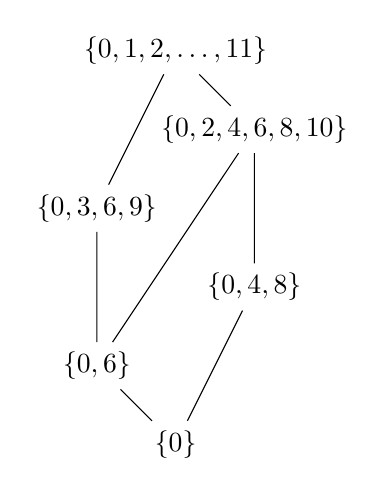
\begin{tikzpicture}
            \node (c1) at (0, 0) {$\{ 0 \}$};
            \node (c2) at (-1, 1) {$\{ 0, 6 \}$};
            \node (c3) at (1, 2) {$\{ 0, 4, 8 \}$};
            \node (c4) at (-1, 3) {$\{ 0, 3, 6, 9 \}$};
            \node (c6) at (1, 4) {$\{ 0, 2, 4, 6, 8, 10 \}$};
            \node (c12) at (0, 5) {$\{ 0, 1, 2, \dots, 11 \}$};

            \draw (c1) -- (c2) -- (c6) -- (c12);
            \draw (c1) -- (c3) -- (c6);
            \draw (c2) -- (c4) -- (c12);
        \end{tikzpicture}
    \end{figure}

    This is called the \term{Hasse diagram} of the subgroup lattice of $C_{12}$.
\end{example}
\chapter{Isomorphic Theorems}

\section{Normal Subgroups}

\begin{definition}[Normal Subgroup]\index{normal subgroup}\label{def:normal-subgroup}
    Let $G$ be a group and $N$ be a subgroup. We say $N$ is a \term{normal subgroup} of $G$, denoted $N \triangleleft G$, if \[
        \forall g \in G, gN = Ng.
    \] Equivalently, if $gNg^{-1} = N$.
\end{definition}

\begin{definition}[Simple Group]\index{simple group}\label{def:simple-group}
    A group $G$ is \term{simple} if it has no nontrivial normal subgroups.
\end{definition}

\begin{example}
    Kernels of group homomorphisms are normal subgroups.

    \begin{proof}
        Let $x \in \ker{\phi}$ for some homomorphism $\phi: G \to H$.

        Then, $\phi(gxg^{-1}) = \phi(g)\phi(x)\phi(g)^{-1} = \phi(g)e\phi(g)^{-1} = e$.

        Therefore, $gxg^{-1} \in \ker{\phi}$.
    \end{proof}
\end{example}

It is important to note that some group are normal under one group but not under another.

\begin{example}
    The alternating group, $A_n$, is normal in the symmetric group, $S_n$.

    This is because $A_n$ is the kernel of the sign homomorphism, which is a normal subgroup by the previous example.

    {~~~}

    For example, consider $S_3$ and $A_3$. \[
        S_3 = \{e, (12), (13), (23), (123), (132)\}, \quad A_3 = \{e, (123), (132)\}.
    \]

    We have $(13)A_3(13) = \{
        (13)e(13), (13)(123)(13), (13)(132)(13)
        \} = \{
        e, (132), (123)
    \} = A_3$.
\end{example}

\section{Isomorphism Theorem}

\begin{definition}[Quotient Group]\index{quotient group}\label{def:quotient-group}
    Let $G$ be a group and $N$ a normal subgroup. Then, we can define the \term{quotient group} $G/N$ as the set of left cosets of $N$ in $G$ with the operation \[
        (gN)(hN) := (gh)N.
    \]
\end{definition}

% \begin{proof}
%     WTS $(gh)N$ is a group. 

%     \begin{enumerate}
%         \item \textbf{Closure:} Let $g_1N, g_2N \in G/N$. Then, \[
%             (g_1N)(g_2N) = (g_1g_2)N \in G/N.
%         \]
%         \item \textbf{Associativity:} Let $g_1N, g_2N, g_3N \in G/N$. Then, \[
%             (g_1N)((g_2N)(g_3N)) = (g_1N)(g_2g_3)N = (g_1g_2g_3)N = (g_1g_2)g_3N = ((g_1N)(g_2N))(g_3N).
%         \]
%         \item \textbf{Identity:} Let $eN \in G/N$. Then, \[
%             (gN)(eN) = (ge)N = gN = (eg)N = (eN)(gN).
%         \]
%         \item \textbf{Inverses:} Let $gN \in G/N$. Then, \[
%             (gN)(g^{-1}N) = (gg^{-1})N = eN = (g^{-1}g)N = (g^{-1}N)(gN).
%         \]
%     \end{enumerate}
% \end{proof}

\begin{theorem}
    $G/N$ is a group if and only if $N \triangleleft G$.
\end{theorem}

\begin{example}
    $A_n$ is normal in $S_n$, so $S_n/A_n$ is a group.

    $A_n$ has $2$ cosets: itself, and the set of all odd permutations. Therefore, $S_n/A_n \cong \Z_2$.

    \begin{center}
        \begin{tabular}{c|c|c}
                      & $A_n$     & $(12)A_n$ \\ \hline
            $A_n$     & $A_n$     & $(12)A_n$ \\ \hline
            $(12)A_n$ & $(12)A_n$ & $A_n$
        \end{tabular}
        $\quad \cong \quad$
        \begin{tabular}{c|c|c}
                & $0$ & $1$ \\ \hline
            $0$ & $0$ & $1$ \\ \hline
            $1$ & $1$ & $0$
        \end{tabular}
    \end{center}

    We have $S_n/A_n \cong \Z/2\Z = \{ 0, 1 \} = \{ -1, 1 \}$.

    Moreover, since $\sgn: S_n \to \{ -1, 1 \}$, we see $S_n/\ker{\sgn} \cong \im{\sgn}$.
\end{example}

\begin{theorem}[The First Isomorphism Theorem]\index{first isomorphism theorem}\label{thm:first-isomorphism}
    Let $G$ be a group, and $\phi: G \to H$ be an homomorphism. Then, \[
        G/\ker{\phi} \cong \im{\phi}.
    \] and the isomorphism is given by \[
        \begin{matrix}
            G/\ker{\phi} & \to     & \im{\phi} \\
            g\ker{\phi}  & \mapsto & \phi(g)
        \end{matrix}
    \]
\end{theorem}

\begin{theorem}[The Correspondence Theorem]\index{correspondence theorem}\label{thm:correspondence}
    Let $G$ be a group, and $N \triangleleft G$. Then, there is a correspondence between the set of subgroups of $G$ containing $N$ and the set of subgroups of $G/N$. \[
        \begin{matrix}
            \left\{ H \le G \mid N \subseteq H \subseteq G \right\} & \longleftrightarrow & \{ K \le G/N \} \\
            H                                                       & \longleftrightarrow & H/N
        \end{matrix}
    \]
\end{theorem}

\begin{figure}[ht!]
    \centering

    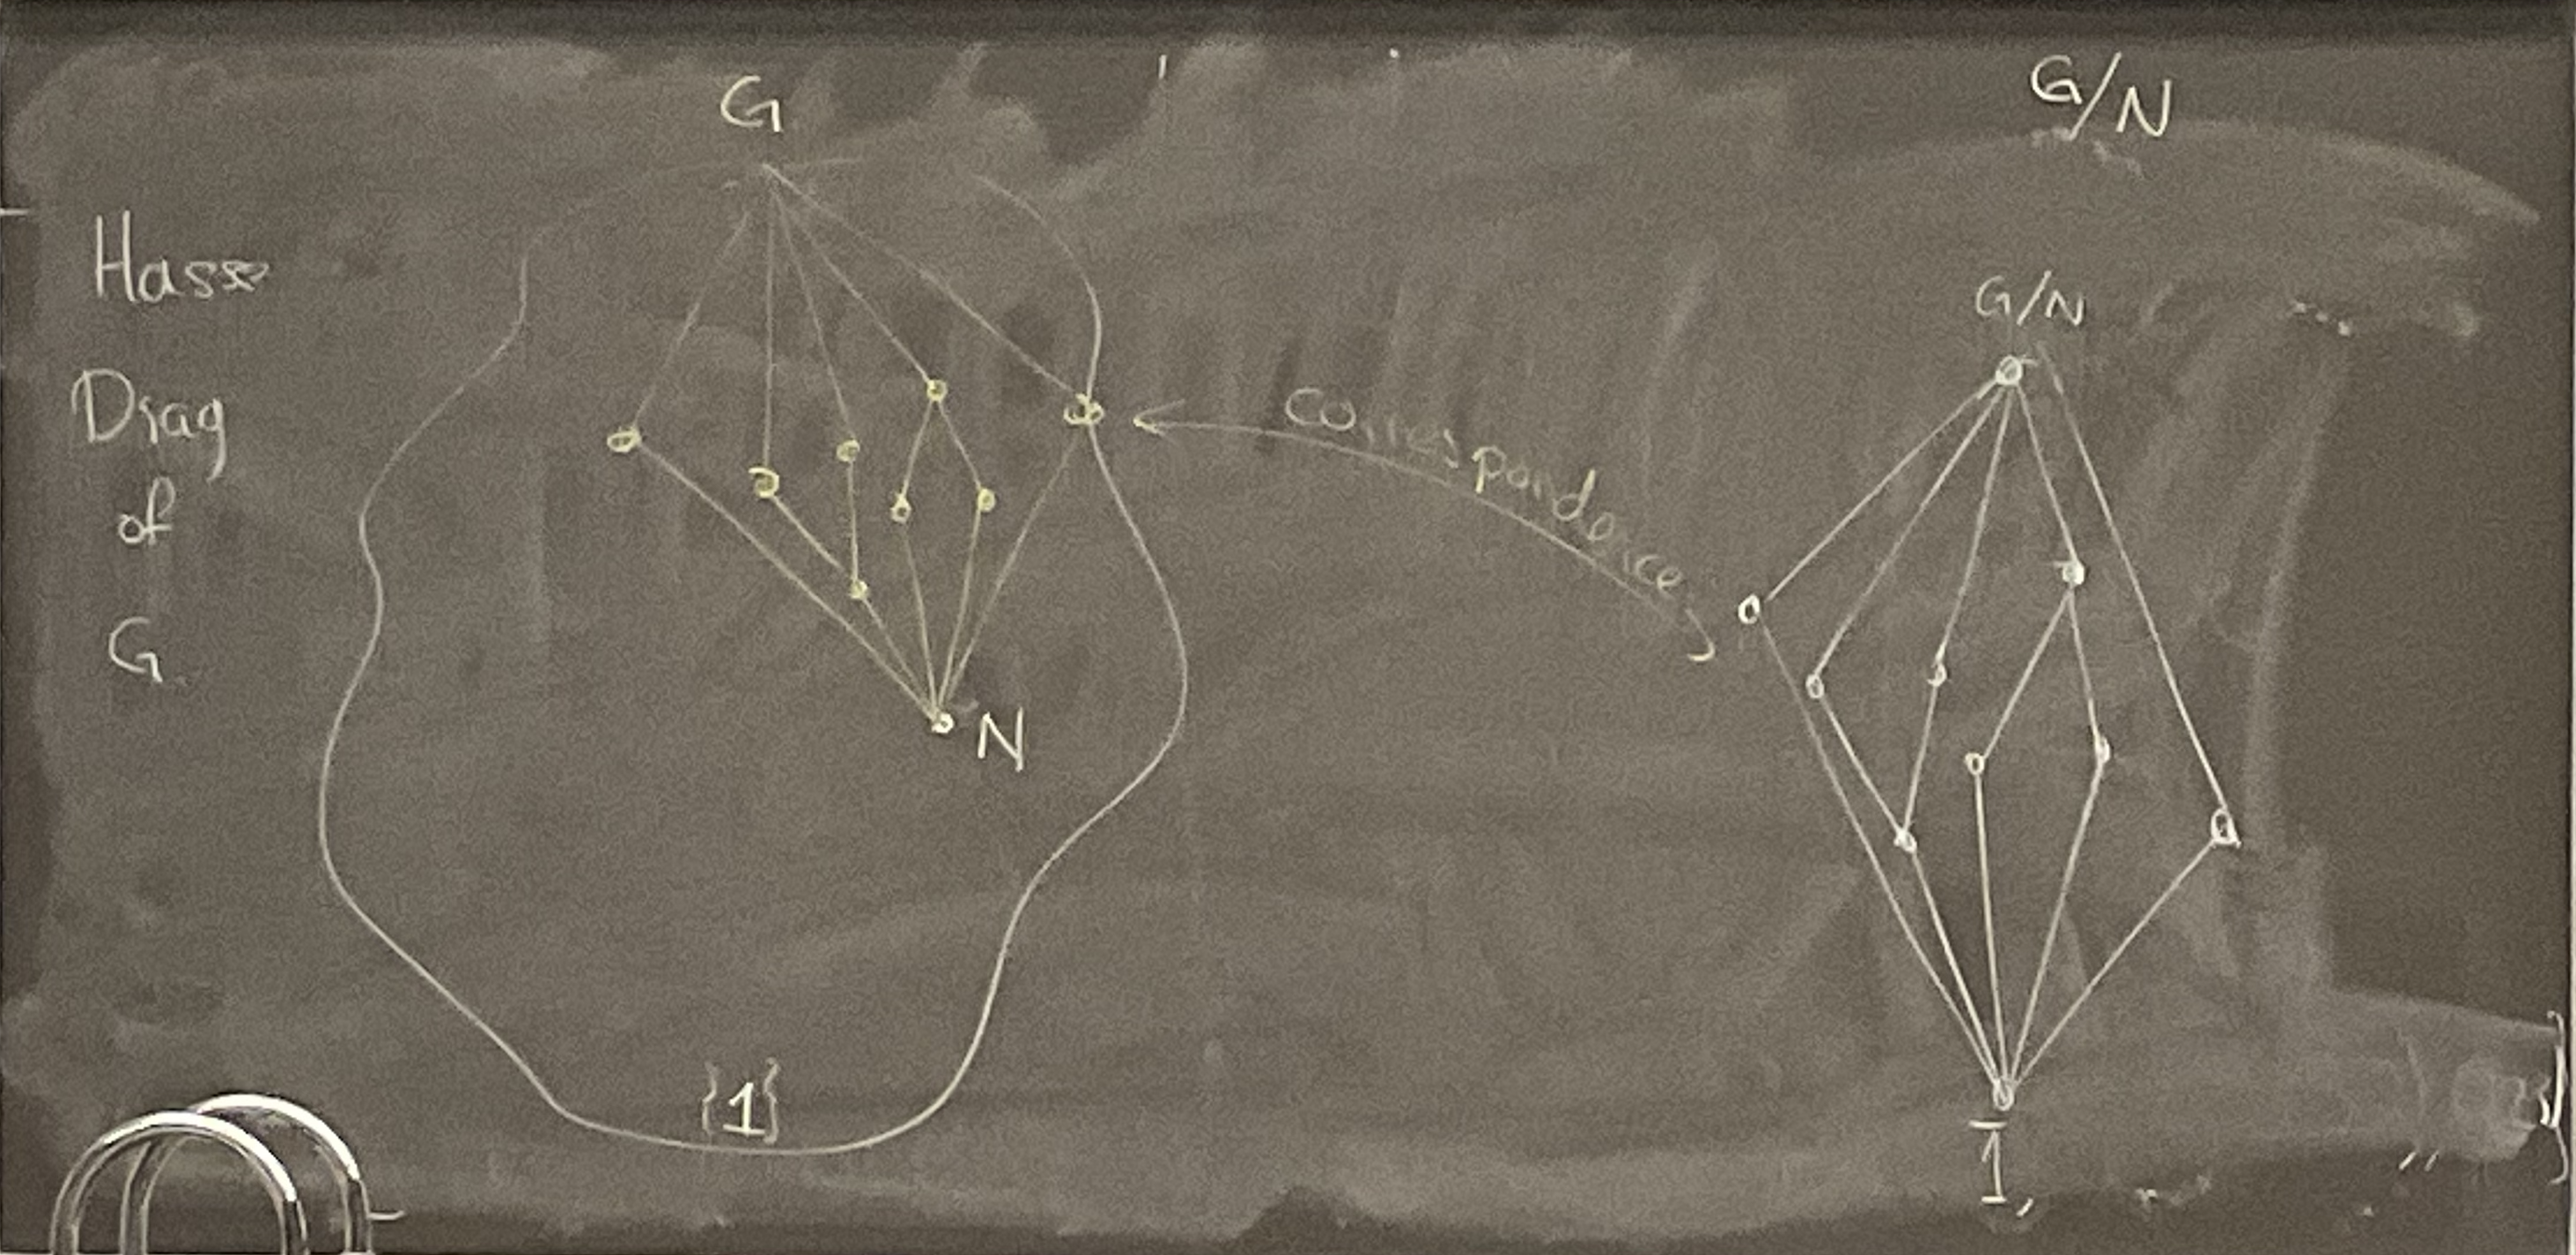
\includegraphics[width=0.67\linewidth]{figures/correspondence-theorem.png}
\end{figure}

The first isomorphism theorem tells us how to reduce the complexity of the group, and the correspondence theorem tells us that we do not loose any information when we do so.

\begin{proposition}
    Let $G$ be a group, and $H$ a subgroup. Then $H$ is normal in $G$ if any only if there exists some homomorphism $\phi: G \to K$ to some group $K$ such that $H = \ker{\phi}$.
\end{proposition}

\begin{remark}
    Sometimes, it is difficult to prove that a subgroup is normal directly. However, if we can find a homomorphism with the subgroup as its kernel, then we can conclude that the subgroup is normal.
\end{remark}

\begin{definition}[Index]\index{index (of a subgroup)}\label{def:index}
    Let $H$ be a subgroup of $G$. The cardinality of $G/H$ is called the \term{index} of $H$ in $G$, denoted $[G:H]$.
\end{definition}

Informally, the index of a subgroup is the number of cosets of the subgroup in the group.

\begin{theorem}
    Let $G$ be a group and $H \le G$ of index $2$. Then, $H$ is normal in $G$.
\end{theorem}

We will construct a homomorphism $\phi: G \to \Z_2$ with $H = \ker{\phi}$, and thus $H \triangleleft G$.

\begin{remark}
    We often construct the homomorphism by manifesting some property of the subgroup.
\end{remark}

\begin{proof}
    Since $[G:H] = 2$, we have $G = H \sqcup g_0H$ for some $g_0 \in G \setminus H$.

    Define a function \[ phi: G \to \{ 1, -1 \} \] by \[
        \phi(g) = \begin{cases}
            1  & g \in H    \\
            -1 & g \in g_0H
        \end{cases}
    \]

    We claim that $\phi$ is a homomorphism. That means to prove $\phi(gh) = \phi(g)\phi(h)$ for all $g, h \in G$.

    In words, this means
    \begin{listu}
        \item $g, h \in H$ implies $gh \in H$

        This follows from the fact that $H$ is a subgroup.

        \item $g, h \notin H$ implies $gh \in H$

        % TODO
        % If $g, h \notin H$, then $g = g_0t_1$ and $h = g_0t_2$ for some $t_1, t_2 \in H$.

        \item $g \in H$ and $h \notin H$ implies $gh \notin H$

        If $g \in H$ and $h \notin H$, then $g \in H$ and $h \in g_0 H$.

        This means $\exists t \in H$ s.t. $h = g_0t$.

        Suppose for contradiction that $gh = g g_0 t \in H$.

        Then, $g_0 = g^{-1} (gh) t^{-1} \in H$, which is a contradiction.
    \end{listu}

    We conclude that $\phi$ is indeed a homomorphism.

    By definition, \[
        \ker{\phi} = \{ g \in G \mid \phi(g) = 1 \} = \{ g \in G \mid g \in H \} = H.
    \]

    Therefore, $H$ is normal in $G$.
\end{proof}

\begin{example}
    These are some examples of normal subgroups we have seen before.

    \begin{listo}
        \item Let $D_n$ be the dihedral group generated by $R$ and $S$. 
        
        $| D_n | = 2n$. 
        
        $\{ 1, R, \dots, R^{n-1} \} \cong C_n$ is a subgroup of index $2$, $[D_n : C_n] = 2$.

        Thus, $\{ 1, R, \dots, R^{n-1} \} \triangleleft D_n$.

        \item Let $\mathcal{R}$ be the group generated by Rubik's cube of $2 \times 2 \times 1$. 
        
        $| \mathcal{R} | = 48$.

        $V_1, V_2, H_1, H_2$ is a subgroup that generates $S_4$, so $[ \mathcal{R} : S_4 ] = 2$.

        Thus, $S_4 \triangleleft \mathcal{R}$.
    \end{listo}
\end{example}

\begin{theorem}
    Let $p$ be a prime number, and $G$ be a group of order $p^2$. Then, $G$ is isomorphic to \[
        C_{p^2} \quad \text{or} \quad C_p \times C_p.
    \]
\end{theorem}

\begin{proof}
    If $G$ is cyclic, then $G \cong C_{p^2}$.

    Suppose $G$ is not cyclic. 

    Let $x \in G$. Since $|x|$ divides $|G| = p^2$ by Lagrange Theorem, we have $|x| \in \{ 1, p, p^2 \}$.

    $|x| = 1$ iff $x = e$, and $|x| \neq p^2$ since $G$ is not cyclic.

    Every non-identity element must have has order $p$.

    {~~~}

    We count the number of $C_p$'s in $G$.

    The only intersections two of these $C_p$'s can have is the identity, $\{ e \}$, since $p$ is prime.

    The count is as follows: \[
        (\text{number of } C_p) \times (p-1) + 1 = p^2.
    \]

    The number of $C_p$'s is \[
        \frac{p^2 - 1}{p-1} = p + 1.
    \]

    \begin{center}
        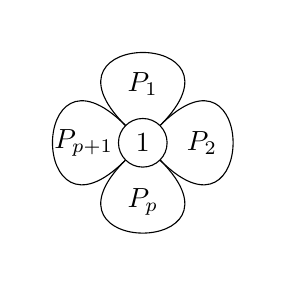
\begin{tikzpicture}
            \node[draw, circle] (1) at (0, 0) {$1$};
            \draw (1) to [in=135, out=45,  looseness=10] (1);
            \draw (1) to [in=45,  out=315, looseness=10] (1);
            \draw (1) to [in=225, out=315, looseness=10] (1);
            \draw (1) to [in=135, out=225, looseness=10] (1);

            \node at (0, 0.75)  {$P_1$};
            \node at (0.75, 0)  {$P_2$};
            \node at (0, -0.75) {$P_p$};
            \node at (-0.75, 0) {$P_{p+1}$};
        \end{tikzpicture}
    \end{center}

    Each of these is a cyclic group of order $p$. 

    Take $g \in G$, $P_i$ the cyclic group generated by $g$. \[
        g P_i g^{-1} = P_j
    \] for some cyclic group $P_j$.

    Let us call $\Phi(g) \in S_{p+1}$ such that \[
        g P_i g^{-1} = P_{\Phi(g)(i)}.
    \]

    In this way we have created a map \[
        \Phi: G \to S_{p+1}.
    \]

    We claim that $\Phi$ is a homomorphism.

    Pick $xy \in G$, $\begin{aligned}[t]
        (xy) P_i (xy)^{-1} &= x(y P_i y^{-1})x^{-1} \\
                           &= x P_{\Phi(y)(i)} x^{-1} \\
                           &= P_{\Phi(x)(\Phi(y)(i))}.
    \end{aligned}$

    Meanwhile, $(xy) P_i (xy)^{-1} = P_{\Phi(xy)(i)}$, so $\Phi(xy)(i) = \Phi(x)(\Phi(y)(i))$ for all $i$.

    Therefore, $\Phi(xy) = \Phi(x) \circ \Phi(y)$.

    {~~~}

    Thus, $\Phi: G \to S_{p+1}$ must satisfy \vspace{-1em} \[ 
        p^2 = | \ker{\Phi} | \cdot | \im{\Phi} |.
    \]

    If $\ker{\Phi} = \{ e \}$, then $| \im{\Phi} | = p^2$.

    This cannot happen, since $p^2$ is not a divisor of $(p+1)!$, the order of $S_{p+1}$.

    This is a violation of Lagrange's Theorem.

    Then, the kernel of $\Phi$ is not trivial.

    {~~~}

    There are elements $x \neq e$ such that \[
        x P_i x^{-1} = P_i \quad \text{for all } i.
    \]

    Suppose $P_i$ does not contain $x$, and consider $y$ a generator of $P_i$. 

    Then, $x y x^{-1} = y^n$ for some $n$. \[
        y^{2n} = (x y x^{-1}) (x y x^{-1}) = x y^2 x^{-1}
    \] 

    Continuing like this, \[
        x y^k x^{-1} = y^{kn}
    \]

    {~~~}

    The powers of $x$, $\{ 1, x, x^2, \dots, x^{p-1} \}$, move the elements of $P_i$ as follows:
    \begin{align*}
        x^2 y x^{-2} & = x (x y x^{-1}) x^{-1} \\
                     & = x y^n x^{-1}          \\
                     & = (x y x^{-1})^n        \\
                     & = (y^n)^n               \\
                     & = y^{n^2}.
    \end{align*}

    Continuing like this, \[
        x^k y x^{-k} = y^{n^k}.
    \]

    {~~~}

    Pick $k = p-1$, we know that $x^{p-1} = x^{-1}$, so \[
        x^{-1} y x = y^{n^{p-1}} = y
    \] by Fermat's Little Theorem.

    \begin{theorem}[Fermat's Little Theorem]\index{Fermat's Little Theorem}
        Let $p$ be a prime number, and $a$ be an integer not divisible by $p$. Then, \[
            a^{p-1} \equiv 1 \mod{p}.
        \]
    \end{theorem}

    This allows us to conclude the following face: \[
        \exists x, y \in G \text{ of order } p \text{ that commute}.
    \]

    Define \[
        \begin{matrix}[rccc]
            \Psi: & \Z/p\Z & \times  & \Z/p\Z \to G \\
                  & (m, n) & \mapsto & x^m y^n
        \end{matrix}
    \]

    \begin{claim}
        $\Phi$ is an isomorphism.
    \end{claim}

    \begin{listu}
        \item \textbf{Injectivity}
        
        $x^m y^n = 1 \implies x^m = y^{-n} \in P_i n P_j = \{ e \}$, where $x \in P_i$ and $y \in P_j$.

        \item \textbf{Surjectivity}
        
        Let $g \in G$. Then, $g = x^m y^n$ for some $m, n \in \Z/p\Z$.

        \item \textbf{Homomorphism}
        \vspace{-1em}
        \begin{align*}
            \Psi(m_1 + m_2, n_1 + n_2) & = x^{m_1 + m_2} y^{n_1 + n_2}     \\
                                       & = x^{m_1} x^{m_2} y^{n_1} y^{n_2} \\
                                       & = x^{m_1} y^{n_1} x^{m_2} y^{n_2} \\
                                       & = \Psi(m_1, n_1) \Psi(m_2, n_2)
        \end{align*}
    \end{listu}

    This completes the proof.
\end{proof}

\subsection{Hasse Diagram of Groups}

Consider the Hasse diagram of $D_6$. There are 2 elements that generate everything, $R$ and $S$. They satisfy $\begin{cases}
    R^6 = e \\
    S^2 = e \\
    SRS = R^5 
\end{cases}$

The elements are \begin{itemize}
    \item $e, R, R^2, R^3, R^4, R^5$
    \item $S, SR, SR^2, SR^3, SR^4, SR^5$
\end{itemize}

To build the Hasse diagram, we need the divisors of $| D_6 | = 12$. Hence, we have \[
    1, 2, 3, 4, 6, 12,
\] same as $C_{12}$. However, since $D_6$ is not cyclic, we do not know if the subgroups of $D_6$ are cyclic.

\subsubsection{Cyclic Subgroups of $D_6$}

% TODO

% See notes P.10. 

% On P.19, $\bar{S}$ means $S \langle R^2 \rangle$, similarly for all other elements with a bar.

\includepdf[pages=-,nup=2x3]{/Users/lance/Downloads/MAT301 S 2024 Lecture 10.pdf}
\chapter{Actions of Groups}

\section{Group Actions}

\begin{definition}[Action]\index{action (of a group)}\label{def:action}
    Let $G$ be a group and $X$ a set. We say $G$ \term{acts on $X$} if there is a map \[
        \begin{matrix}[rccc]
            \cdot: & G \times X & \to     & X \\
                   & (g, x)     & \mapsto & g \cdot x
        \end{matrix}
    \] such that \begin{enumerate}
        \item $e \cdot x = x$ for all $x \in X$.
        \item $g \cdot (h \cdot x) = (gh) \cdot x$ for all $g, h \in G$ and $x \in X$.
    \end{enumerate}
\end{definition}

Associated with an action, there are three important constructions.

\begin{definition}[Orbit]\index{orbit}\label{def:orbit}
    Let $G$ act on $X$. The \term{orbit} of $x \in X$ is the set \[
        \mathcal{O}_x = \{ g \cdot x \mid g \in G \}.
    \]
\end{definition}

\begin{definition}[Stabilizer]\index{stabilizer}\label{def:stabilizer}
    Let $G$ act on $X$. The \term{stabilizer} of $x \in X$ is the set \[
        Stab_x(G) = \{ g \in G \mid g \cdot x = x \}.
    \]
\end{definition}

\begin{example}
    Given a group $G$ we say $G$ acts on itself by conjugation by defining \[
        h^g = C_g(h) = g h g^{-1}.
    \] This is an action. 
    \begin{listu}
        \item $1 \cdot x = 1 \cdot x \cdot 1^{-1} = x$
        \item $C_(C_h(k)) = C_g(hkh^{-1}) = ghkh^{-1}g^{-1} = ghk(gh)^{-1} = (gh) \cdot k = C_{gh}(k)$
    \end{listu}
\end{example}

\begin{definition}[Conjugacy Class]\index{conjugacy class}\label{def:conjugacy-class}
    The orbit under conjugation is called the \term{conjugacy class} of $G$.
\end{definition}

\begin{remark}
    Conjugacy classes is \bred{not a subgroup} of $G$.
\end{remark}

\begin{example}
    Consider $S_3 = \{ e, (12), (13), (23), (123), (132) \}$.

    \begin{minipage}[t]{0.45\linewidth} \begin{listu}
        \item $(12) 1 (12)^{-1} = 1$
        \item $(12) (12) (12)^{-1} = (12)$
        \item $(12) (13) (12)^{-1} = (23)$
        \item $(12) (23) (12)^{-1} = (13)$
        \item $(12) (123) (12)^{-1} = (132)$
        \item $(12) (132) (12)^{-1} = (123)$
    \end{listu} \end{minipage}
    \begin{minipage}[t]{0.45\linewidth} \begin{listu}
        \item $(123) 1 (123)^{-1} = 1$
        \item $(123) (12) (123)^{-1} = (23)$
        \item $(123) (13) (123)^{-1} = (12)$
        \item $(123) (23) (123)^{-1} = (13)$
        \item $(123) (123) (123)^{-1} = (123)$
        \item $(123) (132) (123)^{-1} = (132)$
    \end{listu} \end{minipage}
\end{example}

\begin{example}
    Now consider $S_4$. 

    \begin{minipage}[t]{0.45\linewidth} \begin{listu}
        \item $(12) 1 (12)^{-1} = 1$
        \item $(12) (12) (12)^{-1} = (12)$
        \item $(12) (13) (12)^{-1} = (23)$
        \item $(12) (14) (12)^{-1} = (24)$
        \item $(12) (23) (12)^{-1} = (13)$
        \item $(12) (24) (12)^{-1} = (14)$
    \end{listu} \end{minipage}
    \begin{minipage}[t]{0.45\linewidth} \begin{listu}
        \item $(12) (34) (12)^{-1} = (34)$
        \item $(12) (12)(34) (12)^{-1} = (12)(34)$
        \item $(12) (13)(24) (12)^{-1} = (14)(23)$
        \item $(12) (14)(23) (12)^{-1} = (13)(24)$
        \item $\cdots$
    \end{listu} \end{minipage}

    We can see that in both examples, the cycle structure is preserved under conjugation. This brings to a very important theorem.
\end{example}

\begin{theorem}
    The conjugacy classes of $S_n$ are classified by the cycle structure of the elements.
\end{theorem}

\begin{example}
    Consider $S_4$, it has the following cycle structures: \[
        (a)(b)(c)(d), \quad (ab), \quad (ab)(cd), \quad (abc), \quad (abcd);
    \] which has \[
        1, \quad 6, \quad 3, \quad 8, \quad 6
    \] elements, respectively.
\end{example}

\begin{example}
    Let $G$ be the set of $n \times n$ matrices over $\C$.

    If $\begin{pmatrix} a & b \\ c & d \end{pmatrix}$ is such a $2 \times 2$ matrix that is diagonalizable, then that means there is a basis of eigenvectors $\{ v_1, v_2 \}$.

    Then, \[
        \begin{pmatrix} a & b \\ c & d \end{pmatrix} = Q \begin{pmatrix} \lambda_1 & 0 \\ 0 & \lambda_2 \end{pmatrix} Q^{-1}.
    \] where $Q$ is the change of basis matrix from the standard basis to the basis of eigenvectors.

    That is, \[
        Q = (v_1, v_2) = \begin{pmatrix} v_{11} & v_{12} \\ v_{21} & v_{22} \end{pmatrix}.
    \]

    We see in generalized eigenvectors that we can either conjugate the matrix to Jordan form $\begin{pmatrix} \lambda & 1 \\ 0 & \lambda \end{pmatrix}$, or we can conjugate the matrix to a block diagonal matrix $\begin{pmatrix} \lambda_1 & 0 \\ 0 & \lambda_2 \end{pmatrix}$.

    Consider if we want to answer if $\begin{pmatrix} 1 & 7 \\ 2 & 3 \end{pmatrix}$ and $\begin{pmatrix} 7 & 5 \\ 1 & i \end{pmatrix}$ conjugate, that is, if there exists a matrix $Q$ such that \[
        \begin{pmatrix} 1 & 7 \\ 2 & 3 \end{pmatrix} = Q \begin{pmatrix} 7 & 5 \\ 1 & i \end{pmatrix} Q^{-1}.
    \]

    A na\"ive approach would be to solve for the eigenvalues of the two matrices, and then solve for the eigenvectors; however, this is not the most efficient way, as calculating the eigenvalues of a matrix is a difficult problem.

    We see that the determinant is preserved under conjugation, so the two matrices are not conjugate.

    Now consider $\begin{pmatrix} 1 & 7 \\ 3 & 2 \end{pmatrix}$ and $\begin{pmatrix} 1 & 2 \\ 0 & -19 \end{pmatrix}$. They have the same determinant, but are they conjugate?

    The answer is no. We need the trace to be preserved as well.

    This is because the determinant and the trace are all operations on the eigenvalues of the matrix (the determinant is the product of the eigenvalues, and the trace is the sum), and the eigenvalues are preserved under conjugation.

    \begin{remark}[Characteristic Polynomial]\index{Characteristic Polynomial}
        Consider an $n \times n$ matrix $A$. The characteristic polynomial of $A$, denoted by $p_A(t)$, is the polynomial defined by \[
            p_A(t) = \det{(tI - A)}.
        \] where $I$ denotes the $n \times n$ identity matrix.
    \end{remark}

    Thus, we need to check the characteristic polynomial of the two matrices to see if they are conjugate. The coefficients of the characteristic polynomial are precisely the invariants of the matrix under conjugation.

    The conjugacy classes is a replacement of eigenvalues. 
\end{example}

\section{Orbit-Stabilizer Theorem}

\begin{theorem}[Cauchy's Theorem]\index{Cauchy's Theorem}\label{thm:cauchy}
    Let $G$ be a finite group and $p$ be a prime number. If $p$ divides the order of $G$, then there exists an element $x \in G$ of order $p$.
\end{theorem}

\begin{example}
    Let $n = 15$, and $|D_{15}| = 30 = 2 \cdot 3 \cdot 5$.

    Then, by Cauchy's Theorem, there exists an element of order $2$, $3$, and $5$ in $D_{15}$.
\end{example}

\begin{example}
    Consider $S_7$. We have $|S_7| = 7! = 2^4 \cdot 3^2 \cdot 5 \cdot 7$.

    Then, by Cauchy's Theorem, there exists an element of order $2$, $3$, $5$, and $7$ in $S_7$.
\end{example}

\begin{example}
    Consider $\RR$. We have $|\RR| = 48 = 2^4 \cdot 3$.

    Then, by Cauchy's Theorem, there exists an element of order $2$ and $3$ in $\RR$.
\end{example}

{~~~}

There are two observations to make about conjugation,
\begin{listu}
    \item If $x \in G$ is fixed by the conjugation, that is, $gxg^{-1} = x$ for all $g \in G$, then $x$ is in the center of $G$.

    \item All conjugacy classes are disjoint. 
\end{listu}

\begin{figure}[ht!]
    \centering
    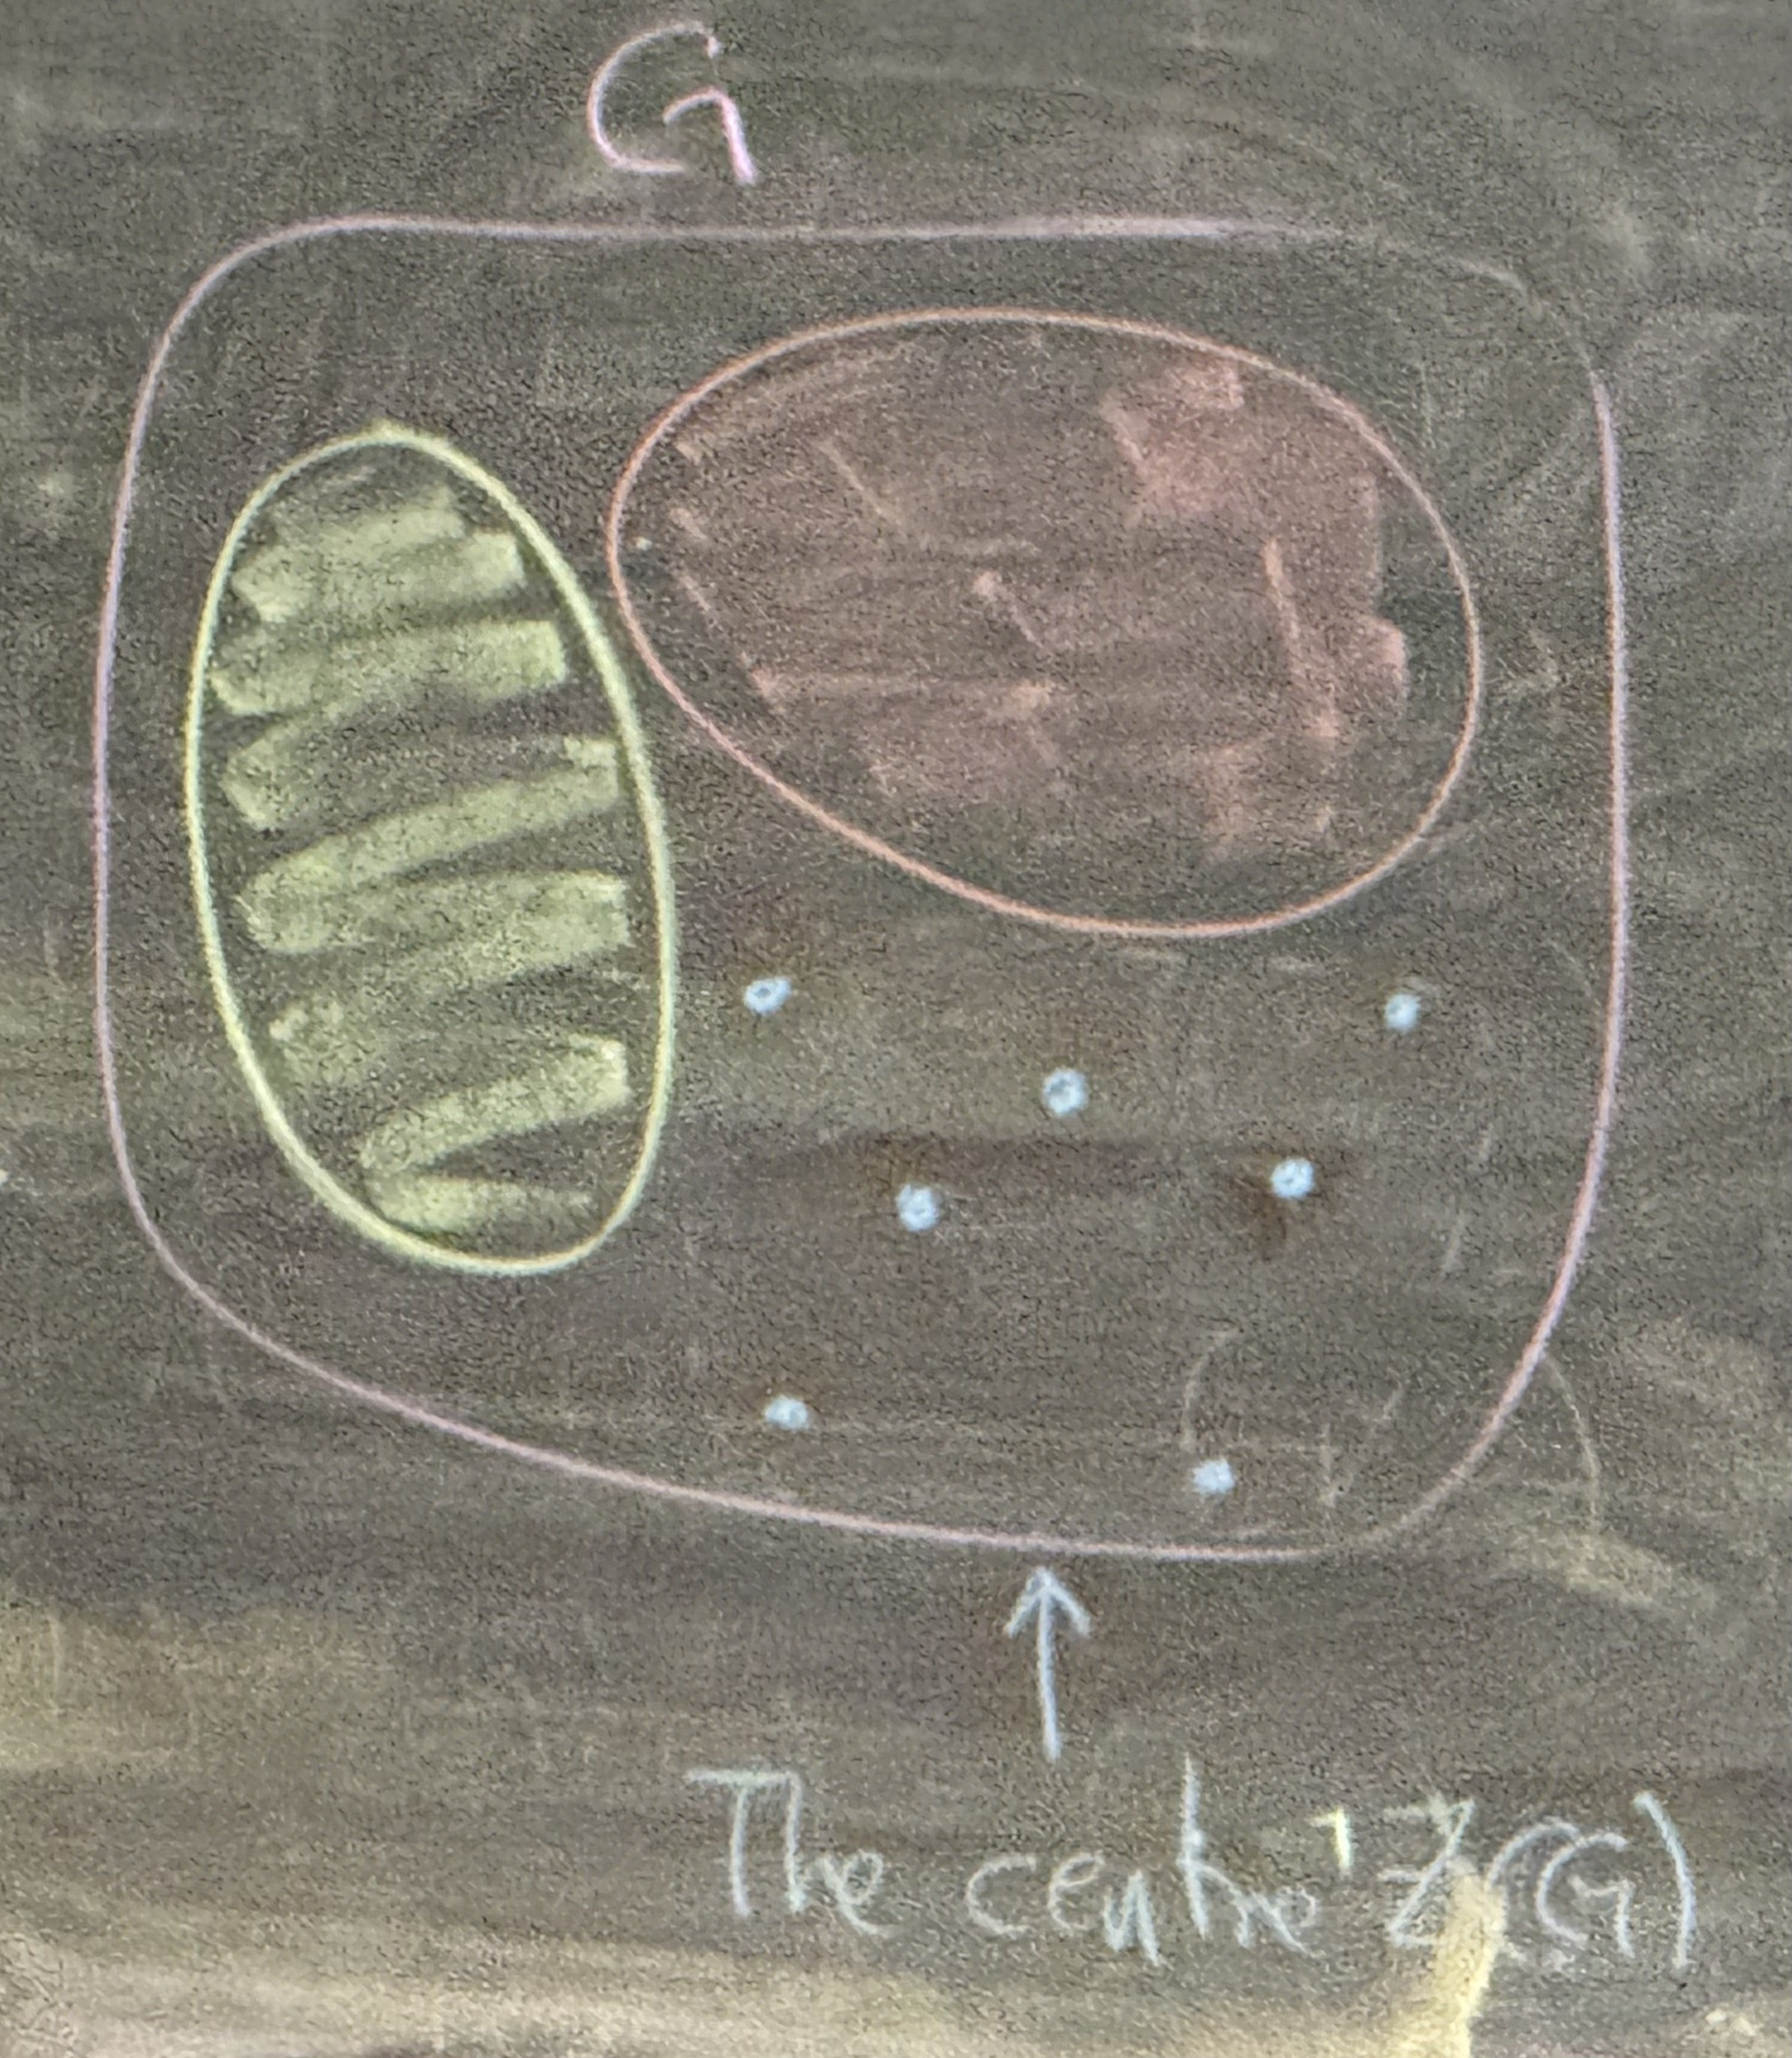
\includegraphics[width=0.2\linewidth]{figures/conjugacy-class.jpg}
\end{figure}

From this we get \[
        |G| = |Z(G)| + \sum_{\substack{x \notin Z(G) \\\text{without repeating conjugacy classes}}} | Conj(x) |.
\] This equation is called the \term{class equation}\index{class equation}.

\begin{theorem}[Orbit-Stabilizer Theorem]\index{orbit-stabilizer theorem}\label{thm:orbit-stabilizer}
    Let $G$ be a finite group acting on a set $X$. Then, for any $x \in X$, \[
        | G | =  | \mathcal{O}_x | \cdot | Stab_x(G) |.
    \]

    It can also be written as \[
        G / Stab_x(G) \cong \mathcal{O}_x.
    \]
\end{theorem}

\begin{listu}
    \item $\mathcal{O}_x$ are all elements of $X$ I can reach from $x$. 
    \item $Stab_x(G)$ are all elements of $G$ that fix $x$ (i.e. $g \cdot x = x$).
\end{listu}

\begin{proof}
    Let $x \in X$ and $\mathcal{O}_x = \{ h \cdot x \mid g \in G \} = \{ x_1, x_2, \dots, x_k \}$.

    We make a table \begin{table}[ht!]
        \centering
        \begin{tabular}{c|c}
                      & Elements $g$  s.t. $g \cdot x = x_i$                       \\ \hline
            $x = x_1$ & $g \cdot x = x$ I have written the elements of $Stab_x(G)$ \\ \hline
            $x_2$     & $g \cdot x = x_2$                                          \\ \hline
            $\vdots$  & $\vdots$                                                   \\ \hline
            $x_k$     & $g \cdot x = x_k$
        \end{tabular}
    \end{table}
    % \begin{figure}[ht!]
        % \centering
    \begin{center}
        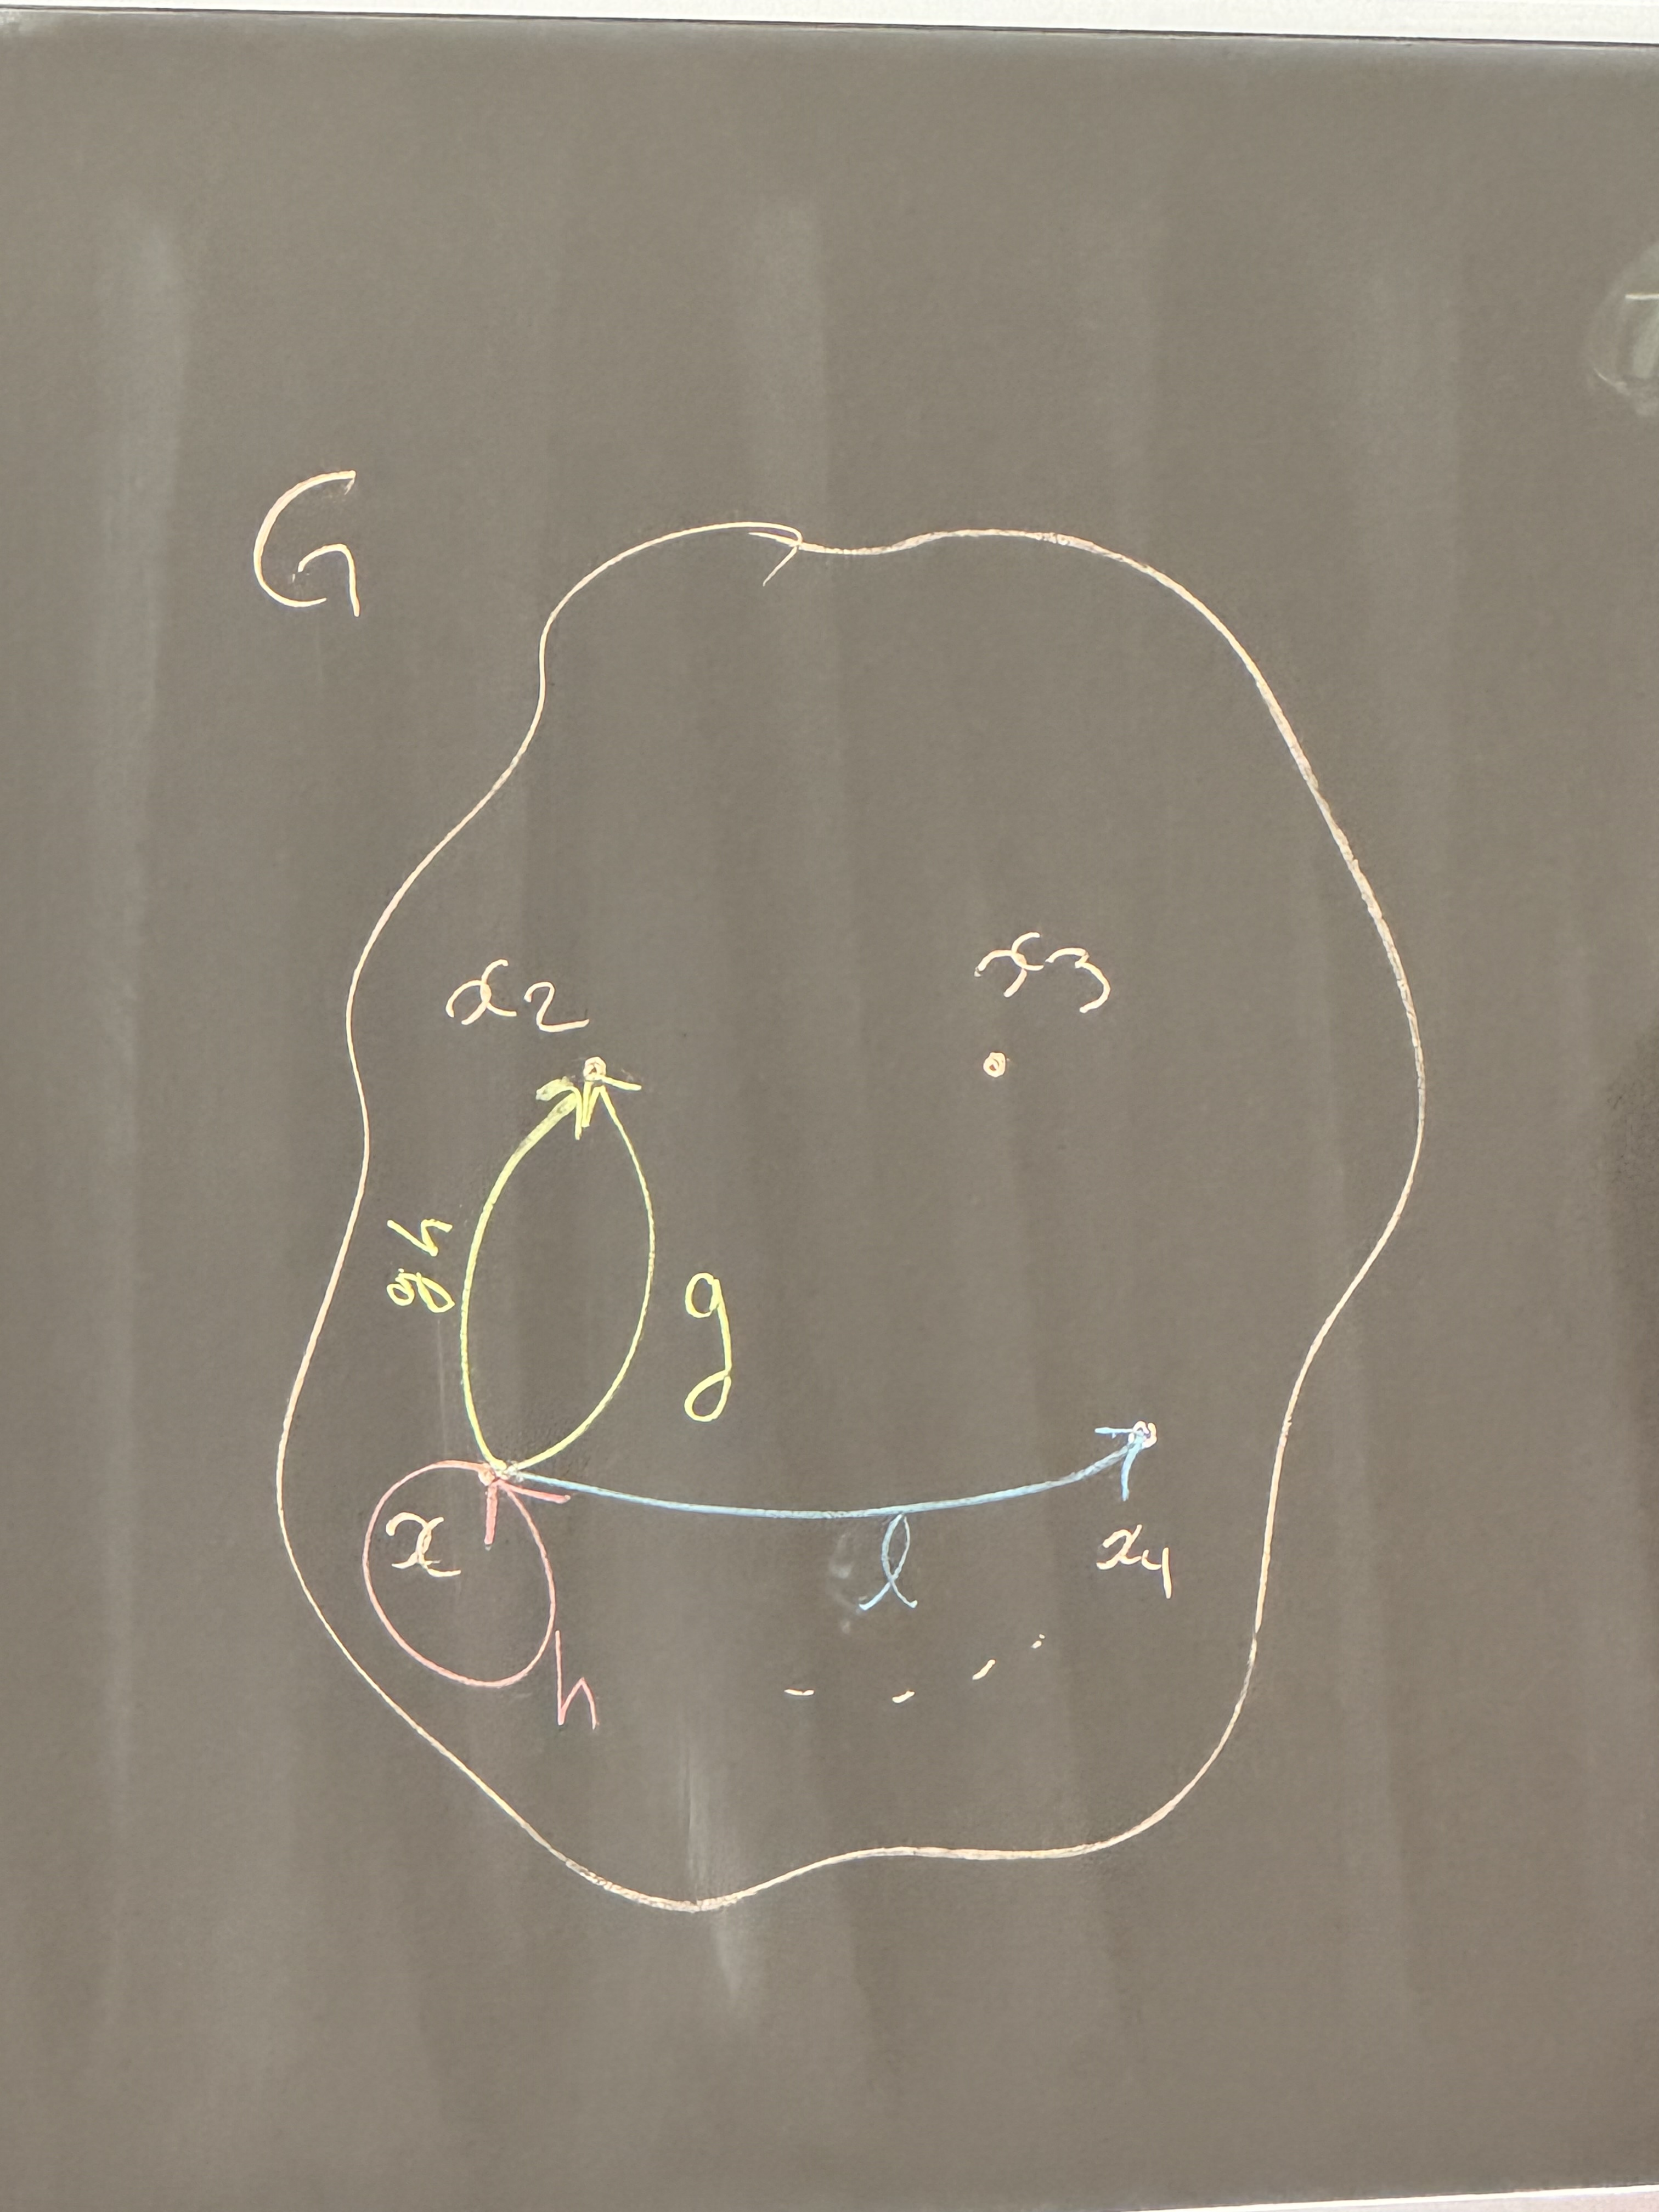
\includegraphics[width=0.2\linewidth]{figures/orbit-stabilizer-proof.jpg}
    % \end{figure}
    \end{center}

    We can write \[
        gh
    \] with $h \in Stab_x(G)$ and $g \cdot x = x_2$ and get \[
        gx \cdot x = g \cdot (h \cdot x) = g \cdot x = x_2
    \]

    With this we see that $g Stab_x(G)$ satisfies to only one element of $\mathcal{O}_x$. This is a coset of $Stab_x(G)$.

    % \begin{table}[ht!]
    %     \centering
    %     \begin{tabular}{c|c}
    %                   & Elements $g$  s.t. $g \cdot x = x_i$                       \\ \hline
    %         $x = x_1$ & $g \cdot x = x$ I have written the elements of $Stab_x(G)$ \\ \hline
    %         $x_2$     & $g \cdot x = x_2$                                          \\ \hline
    %         $\vdots$  & $\vdots$                                                   \\ \hline
    %         $x_k$     & $g \cdot x = x_k$
    %     \end{tabular}
    % \end{table}

    However, there may be an $x_i$ who produces more than one cosets, so we cannot make the claim yet.

    % \begin{figure}[ht!]
        % \centering
    \begin{center}
        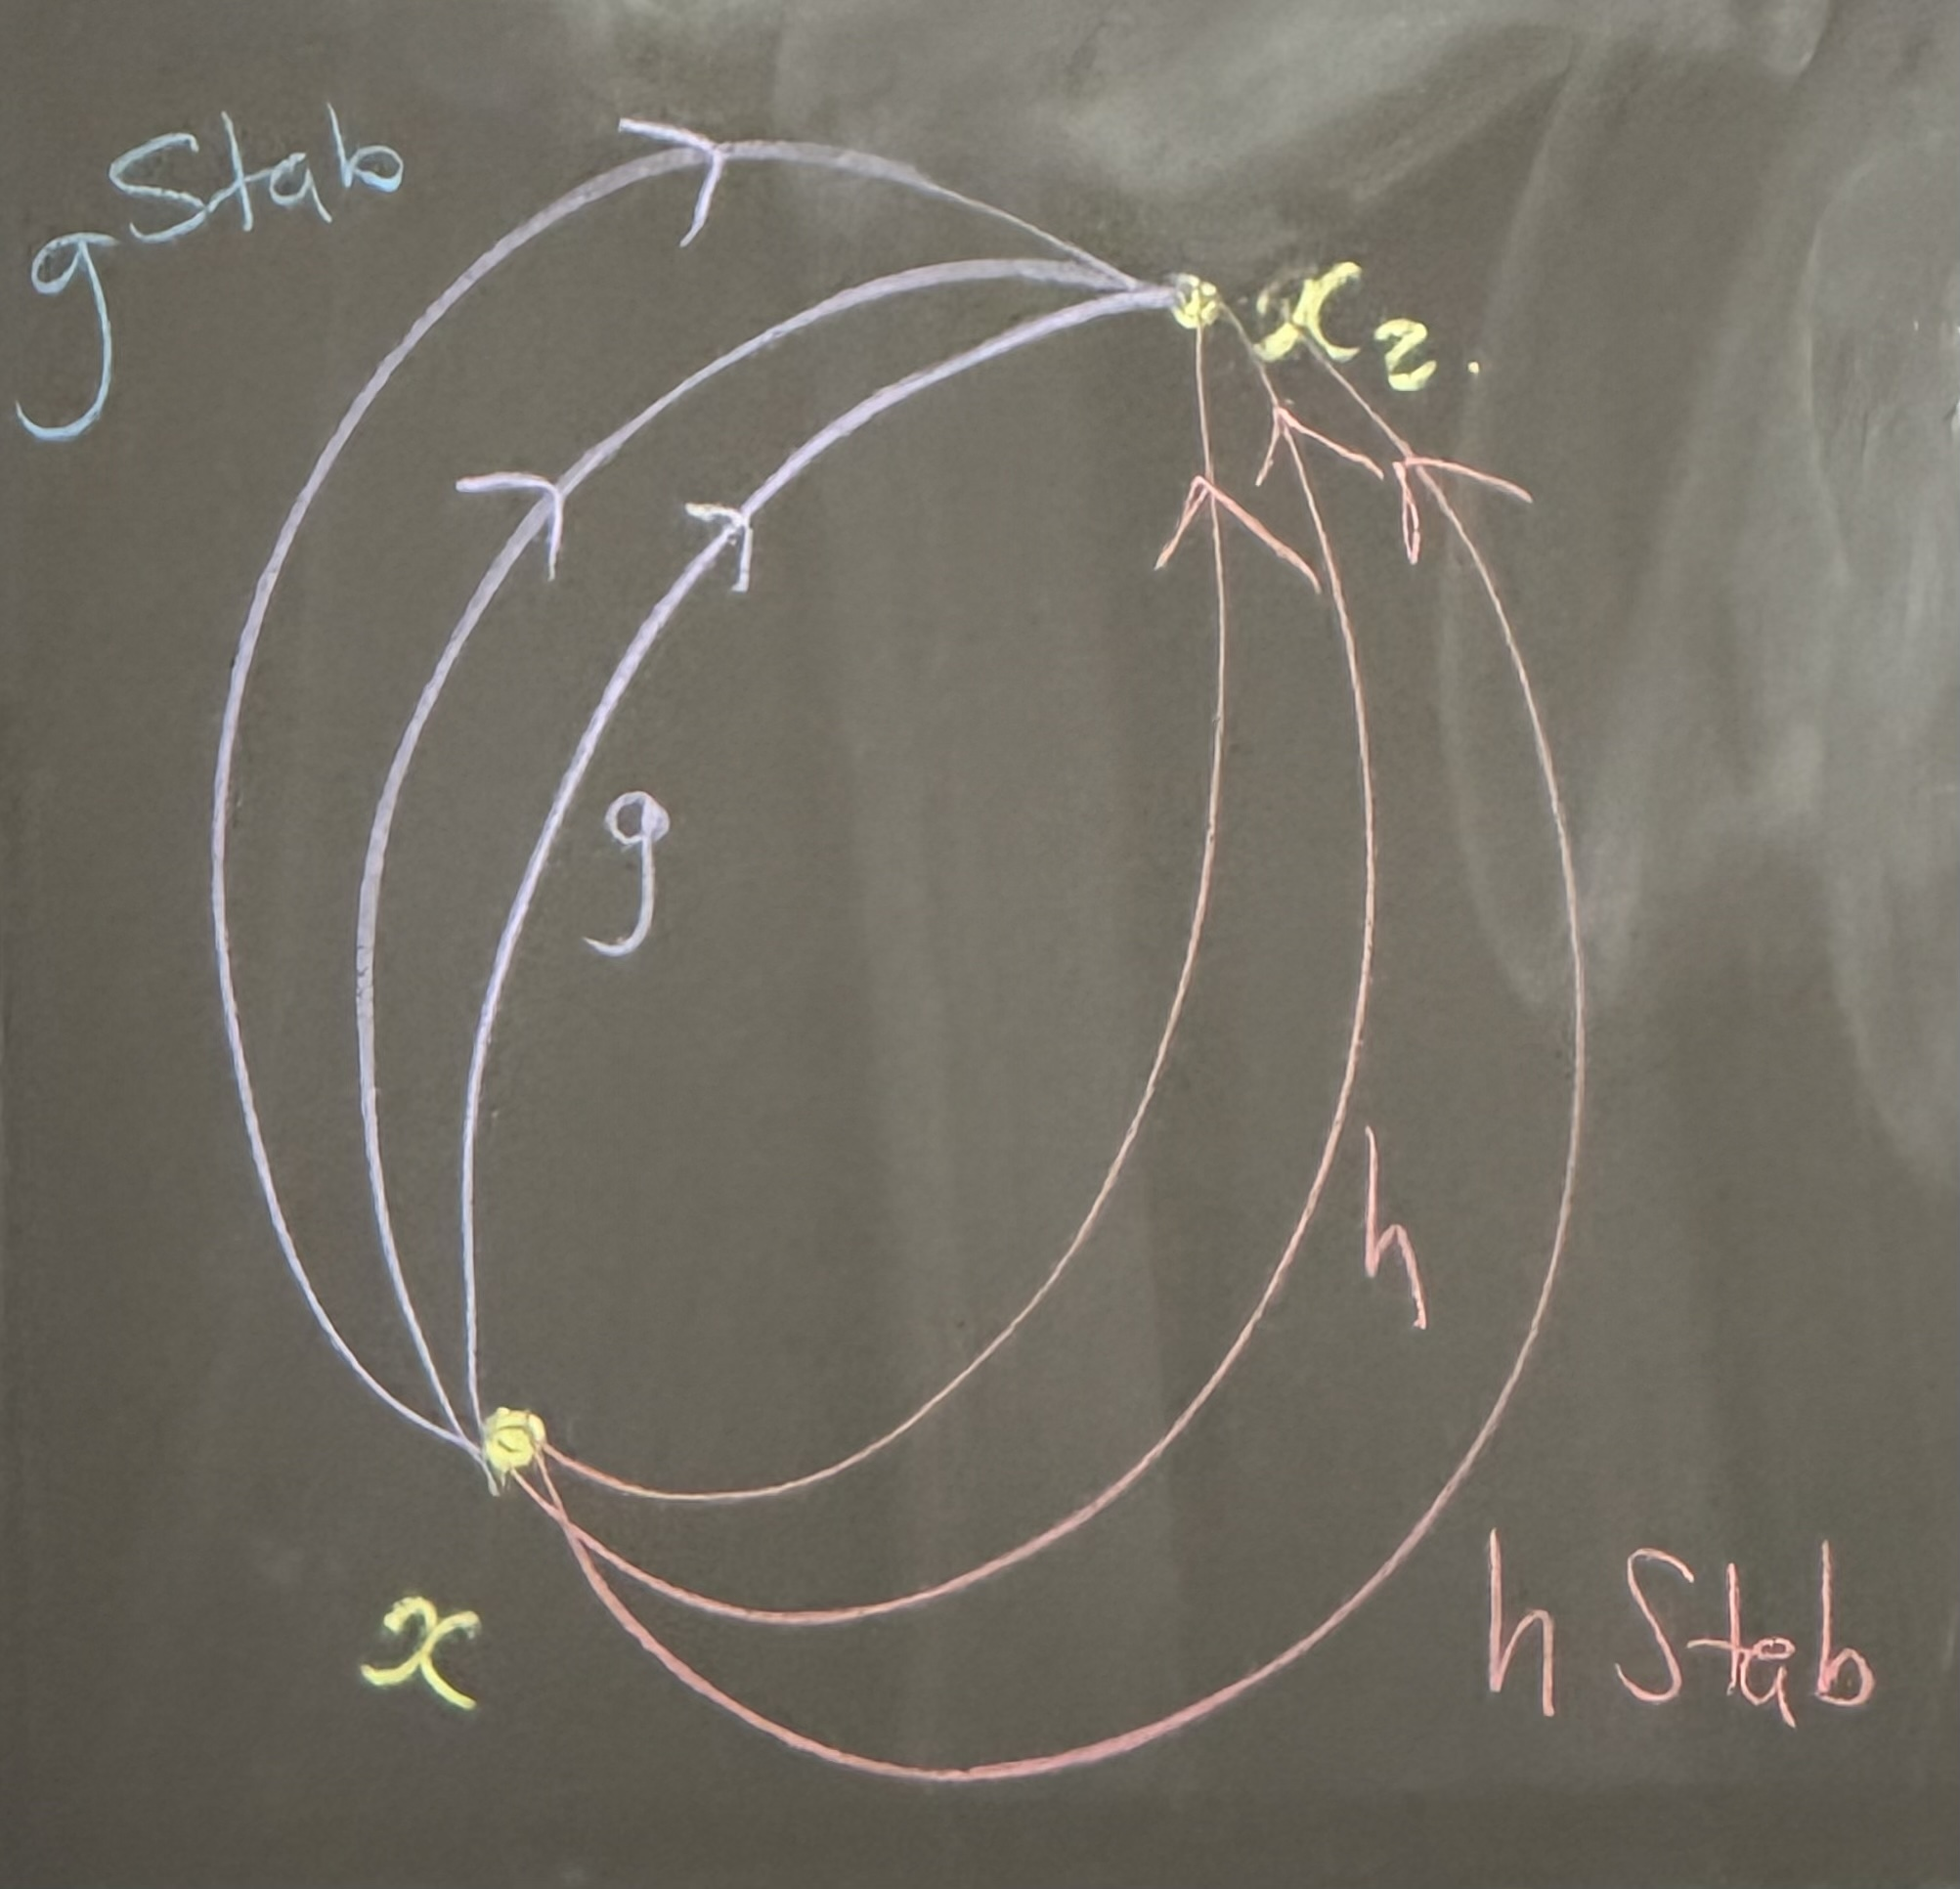
\includegraphics[width=0.2\linewidth]{figures/orbit-stabilizer-proof-2.jpg}
    \end{center}
    % \end{figure}

    If a row contains $g$ and $h$, then they must be in the same coset of $Stab_x(G)$.

    Indeed, $g^{-1} \cdot (h \cdot x) = g^{-1} \cdot x_2 = x$, thus $g^{-1} h \in Stab_x(G)$.

    This is the criteria for two elements to be in the same coset. Thus $g$ and $h$ are in the same coset.
    % We consider the path $x \overrightarrow{g} x_2 \overrightarrow{h} x$. 

    Then $|G| = \underset{Number of rows}{| \mathcal{O}_x |} \cdot \underset{Number of elements in each row}{| Stab_x(G) |}$.
\end{proof}

\begin{example}
    Consider the proof for \hyperref[thm:cauchy]{Cauchy's Theorem}.

    \begin{proof}
        Suppose we know the result for two cases:

        \begin{listo}
            \item If $H$ is abelian
            \item If $|H| < |G|$
        \end{listo}

        Let us use the class equation \[
            |G| = |Z(G)| + \sum_{\substack{x \notin Z(G) \\\text{without repeating conjugacy classes}}} | Conj(x) |.
        \]

        We know $p \mid |G|$. We have two possibilities: \begin{enumerate}
            \item $p \mid |Z(G)|$

            In this case, we are done.

            \item $p \not\mid |Z(G)|$

            We consider the conjugacy classes. 

            Known that $|G| = |Conj(x)| \cdot |Stab_x(G)|$ by the \hyperref[thm:orbit-stabilizer]{Orbit-Stabilizer Theorem}, and $|Stab_x(G)| < |G|$, so we fall under the second case ($|H| < |G|$).

            The only case remaining is if $p \div |Conj(G)|$ and $p \not\div |Z(G)|$.

            However, this is not possible, as $|Conj(G)| = |G| - |Z(G)|$, and $p \not\mid |Z(G)|$. 
        \end{enumerate}
    \end{proof}
\end{example}

\part{Appendices}

\chapter*{Bibliography}
\addcontentsline{toc}{part}{Bibliography}
\nocite{*}
\printbibliography[heading=bibempty]

\cleardoublepage
\phantomsection
\setlength{\columnsep}{0.75cm}
\addcontentsline{toc}{part}{Index}
\printindex

\end{document}